\section{Introduction}

Advancements in spacecraft technology accelerate discovery in Earth and space sciences; faster reorientation and ultra-quiet jitter-free operation for space observatories and optical links have the potential to transform the rate and quality of data obtained for scientific investigation \cite{Arnon1998a, Ruiter2013a}. Scientific needs drive exceptionally stringent spacecraft pointing and control requirements, which in turn demand new strategies for space vehicle design and control \cite{Sirlin1987a, Rao1994a}.
The strategy proposed here uses existing appendages (solar arrays) with distributed actuation to achieve high-precision attitude control. \Glsfirstplural{SASA}, which employ distributed piezoelectric material actuators, provide high accuracy and bandwidth for spacecraft attitude control, thereby supporting quiet operation for high-precision scientific instruments. Additionally, the dual use of the same spacecraft component, i.e.,~solar arrays, for power generation and precision attitude control reduces payload delivery costs.

% new paragraph
A unique capability of the proposed SASA pointing architecture is to perform attitude slewing maneuvers in addition to suppressing structural vibrations. 
Although the current bending limit of the arrays bounds the magnitude of the attitude maneuvers to the order of milli-radians or arc minutes, these advancements are important for high precision pointing.
After the pointing target has been acquired, the SASA control system performs small-scale reorientations and pointing stability in the presence of jitter disturbances.

Strain-actuated solar arrays for precision pointing will require the arrays to behave more like a flexible structure than a rigid one. Space structures by necessity are extremely lightweight and flexible, but vibrations from reaction wheel assemblies, reorientation maneuvers, and other disturbances degrade performance.
There has been previous work to handle this issue, including the extensively-studied topic of control-structure interaction \cite{Rao1994a, Meckl1994a}.
However, most of these works have led to design guidelines based on the primary goal of damping out vibrations \cite{Crawley1987a, Manning1991a}.
In contrast, the primary goal here is to control the spacecraft orientation. In the integrated design and control study presented here we seek to utilize the flexible body dynamics to our advantage to provide new levels of system performance.

\Glsfirstplural{PEMA} \cite{Pan1992a, Hubbard1992a, Hwang1993a} are a proven solution for distributed actuation \cite{Alvarez-Salazar1999a, Bailey1985a}. Applying voltage across PEMAs bonded to or embedded within structures induces strain, causing the structure to deform (bend, twist, elongate, or contract depending on design). PEMA-based intelligent structures outperform conventional point-actuated structures \cite{Rao1994a, Dimitriadis1991a}, in terms of mass, fast dynamic response, and high precision \cite{Pinkerton1996a}. Although piezoelectric actuators have been used for structural active damping, they have not been used for slewing control of structures due to their small stroke. The proposed SASA architecture, however, does not slew the array structure about a revolute joint, but bends it to slew the bus using conservation of angular momentum. In this way, the SASA system implements the novel functionality of small-scale attitude control. Since there are small strain limits on array bending, the small PEMA stroke does not limit this application. Furthermore, the use of piezoelectric actuators allows for quiet operation for sensitive instruments.

The distributed actuation of intelligent structures provides tremendous design flexibility. This opens up new opportunities for system performance, but also increases design difficulty \cite{Pinkerton1996a, Fowler2012a}. The co-design work presented here considers not only the design of the actuator system, but also of a distributed structure for optimal active performance. Furthermore, the use of open-loop distributed control allows us to obtain insights for actuator placement and to investigate limits of performance.

In most previous co-design studies, the physical aspects of the system design have been managed in a very simplified manner. For example, physical system (plant) design decisions have often been limited to actuator placement \cite{Fanson1990a, Li2013a}. Many co-design studies have used simplified plant models \cite{Smith1992a, Dimitriadis1991a, Grandhi1989a, Allison2013d} that do not support exploration of changes to distributed geometric structural design, preventing full exploitation of the design synergy between structural tailoring and distributed control system design. A more ideal co-design method supports changes to distributed structural properties (e.g.,~changing structural shape affects how inertial and stiffness properties vary spatially). Structural tailoring coupled with control design has long been recognized as an important, yet formidable problem \cite{Belvin1990a}. Although there are examples of tailoring passive system dynamics to work optimally with active control using lumped plant stiffness, damping, and mass parameters as design variables \cite{Smith1992a}, these methods cannot be extended to distributed parameter systems.

To summarize, much is known regarding the design of control systems and actuators for intelligent structures, but only if the structural design is held fixed. A few examples of fully-integrated design exist, but only with simplified treatment of structural design. Since the proposed SASA pointing architecture involves inherent dynamic coupling between control actuation and flexible structural dynamics, it is a good case for a co-design study. In this work, distributed geometry---specifically, distributed array structure thickness---is optimized simultaneously with distributed moment control of the array structure.

An initial study of the SASA concept was performed previously, focusing on attitude control, to demonstrate its feasibility. It was shown that the spacecraft bus orientation can be controlled by the appropriate bending of the arrays using a \glsfirst{PRBDM}. A more recent study has further developed realistic feedback control systems suitable for SASA architectures \cite{Herber2014c, Salazar2016a, Yu2005a}.
An earlier version \cite{Chilan2016a} of this work introduced the use of Euler-Bernoulli beam theory for a physically consistent description of the array dynamics, and the nonlinear \glsfirst{PDE} model is implemented using Galerkin approximating functions \cite{Bisplinghoff1996a, Junkins1993a, Paranjape2013a}. In the model, piezoelectric actuation is represented by a distributed moment on the array. The model also accounts for the elastic and inertial properties of the actuators. In the spacecraft slewing and pointing maneuvers considered here, the array bending displacement is small. This enables reasonable accuracy when using a linearized bus-array model. Based on this linear model, we present parametric studies that 1) help determine  performance limits, and 2) provide insight into the resulting array designs.

The use of open-loop controls and distributed optimization parameters, e.g.,~voltage and array thickness, allows for solutions that make limited assumptions on the control or physical architecture. This aids in the exploration of ultimate system performance limits \cite{Allison2014b}. Although there may be practical constraints for feedback control system implementation, the resulting co-design solutions can provide important insights into how to design the physical array structure such that it performs optimally as an actively controlled system, capitalizing on synergy between physical- and control-system design \cite{Deshmukh2015a}.

The primary objectives of this work are to demonstrate the feasibility of the SASA attitude control architecture on a representative spacecraft system, to determine the optimal designs of the distributed array structure and controls, and to reveal qualitative design insights for intelligent structures with distributed geometric design. 

This chapter is organized as follows. The models for the bus-array system, distributed composite array structure, distributed control, and PRBDM are presented in Sec.~\ref{sec:ch7:modeling}. The formulation for the combined design of the distributed array structure and distributed control is presented in Sec.~\ref{sec:ch7:formulation}. Analytical results based on PRBDM theory and numerical results of the co-design studies are discussed in Sec.~\ref{sec:ch7:results}. Results include the analysis of the optimal design tradeoff for the array structure, the optimal placement of segmented piezoelectric actuators, and parametric studies on passive damping and jitter disturbance.

\section{Modeling of the Strain-Actuated Solar Arrays and Rigid Spacecraft Bus\label{sec:ch7:modeling}}

The modeling approach used here is based on the recent work on aircraft dynamics with flexible, articulated wings~\cite{Paranjape2012a} (see Ref.~\cite{Nakka2016a} for details).
The spacecraft motion is modeled as an \glsfoo[noindex]{ODE} of a simple cylinder, and the solar array structure is modeled as a PDE of a composite beam with thickness that can vary along its length.

\begin{figure}[t]
\centering

\begin{subfigure}[b]{0.495\columnwidth}
\centering 
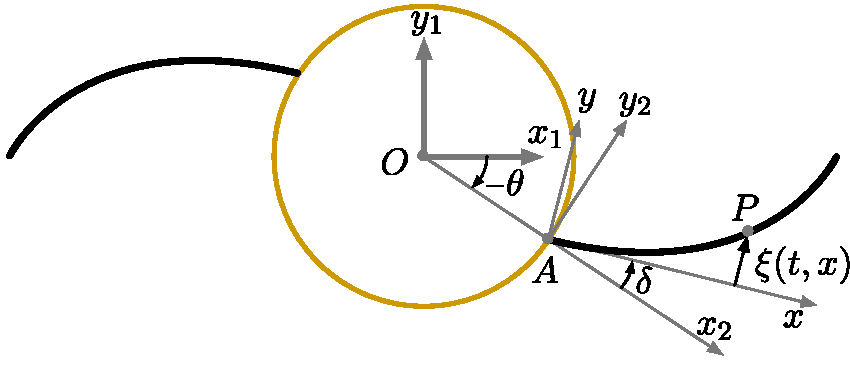
\includegraphics[height=1.2in]{../ch7/figures/coordinate-2}
\caption{Beam theory model.}\label{fig:ch7:coordinate}
\end{subfigure}%
\begin{subfigure}[b]{0.495\columnwidth}
\centering 
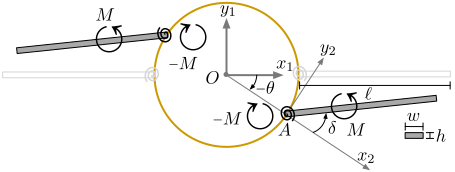
\includegraphics[height=1.2in]{../ch7/figures/prbdm-2}
\caption{Lumped parameter model.}\label{fig:ch7:prbdm}
\end{subfigure}%

\caption{Illustration of the two modeling approaches used to gain design insights. \label{fig:ch7:models}}
\end{figure} 

\subsection{Partial Differential Equation Model \label{sec:ch7:beam}}
Here we assume that actuation is effected only through solar array strain actuators that produce strain at the solar array structure surface, resulting in array bending and a distributed moment due to strain actuator surface forces. The strain actuators do not interact with anything external to the spacecraft system, so the total system momentum must be conserved. Therefore, for a generally \glsfirst{CCW}  movement of the solar array, the bus (\gls{angle}) will rotate in the opposing CW direction allowing for attitude changes. This is evident in both the illustration of the beam theory coordinate system in Fig.~\ref{fig:ch7:coordinate} and its comparable PRBDM lumped parameter model in Fig.~\ref{fig:ch7:prbdm}.

\subsubsection{Coupled ODE-PDE Dynamic Model}

The coordinate systems used for the derivation of the Lagrangian of the system are shown in Fig.~\ref{fig:ch7:coordinate}. The model has two arrays with asymmetric actuation. Let the radius of the spacecraft body be \gls{radius}, and the spacecraft body rotation angle about origin $O$ be $\theta$. In deriving the equations of motion, it is assumed that the deflections \gls{deflection} due to bending are small and the beam has no longitudinal velocity.

The mass moment of inertia of the spacecraft bus is $\gls{massinertia}_{\gls{nottheta}}$. The total length and width of the solar array are represented by \gls{length} and \gls{width}. The mass per unit length of the composite beam is denoted \gls{massR} and the total rigidity is $\gls{totalE}\gls{totalI}$. The further details of the structural model are discussed in Sec.~\ref{sec:ch7:structural}.

The moment applied on the array is \gls{moment} over the locations where a piezoelectric actuator is bonded; a small actuation gap (0.5 cm) was applied at the root and the tip to satisfy the boundary conditions. Using the explicit generalization for the hybrid coordinate systems approach, the equations of motion were derived in Refs.~\cite{Nakka2016a, Chilan2017a}.
\noindent The applied boundary conditions specify zero deflection and slope of the deflected beam at the root, and no external force or moment at the free end.

The proposed SASA architecture is envisioned for high-precision pointing control. To maintain the structural integrity of the arrays and to take into account actuator limitations, bounds are defined for the array strain and control magnitude, which in turn limit array displacements to small values. Therefore, a linearized bus-array system can still predict the dynamics with sufficient accuracy (see Ref.~\cite{Chilan2017a} for details).
While the linear model does not approximate large array displacements accurately, displacements in our tests are small, and linearization  makes the integrated structural and control optimization problem more tractable. This allows to conduct various parametric studies, which support the focus of this work on design methods and design insight. The following linearized equations are now used, and the boundary conditions remain the same:
\begin{gather}
\begin{aligned}
\int_{0}^{\ell} \bm{[M_{sl}]} \begin{bmatrix} \ddot{\theta} \\ \ddot{\xi} \end{bmatrix}d\gls{xspatial} +  \begin{bmatrix} 0 \\ \int_{0}^{\ell} (2EI \xi^{\glsfirst{altderiv}''} +2 \gls{damping} EI \dot{\xi}^{''})^{''} dx\end{bmatrix} = \begin{bmatrix} \glsplural{dynd} \\ \int_{0}^{\ell} 2 M^{''} dx \end{bmatrix}
\end{aligned}\label{eq:ch7:PDEdynamics_linear}\\
\begin{gathered}
\text{where:} \quad \bm{[M_{sl}]} = \begin{bmatrix}m_{11}(\xi) & m_{12}\\ m_{12} & m_{22} \end{bmatrix}=\begin{bmatrix} \left(J_{\theta}/\ell + 2\left (m_{R}\left(x+r\right)^2 \right)  \right) & 2m_{R}\left(x+r \right) \\ 2m_{R}\left(x+r \right) & 2m_{R} \end{bmatrix} \\
\end{gathered} \notag
\end{gather}

\noindent The term $\mu$ is used to model the structural damping in the solar array. A disturbance $d(t)$ acts on the bus as a torque input. 

\begin{figure}[t]
\centering

\begin{subfigure}[b]{0.49\columnwidth}
\centering 
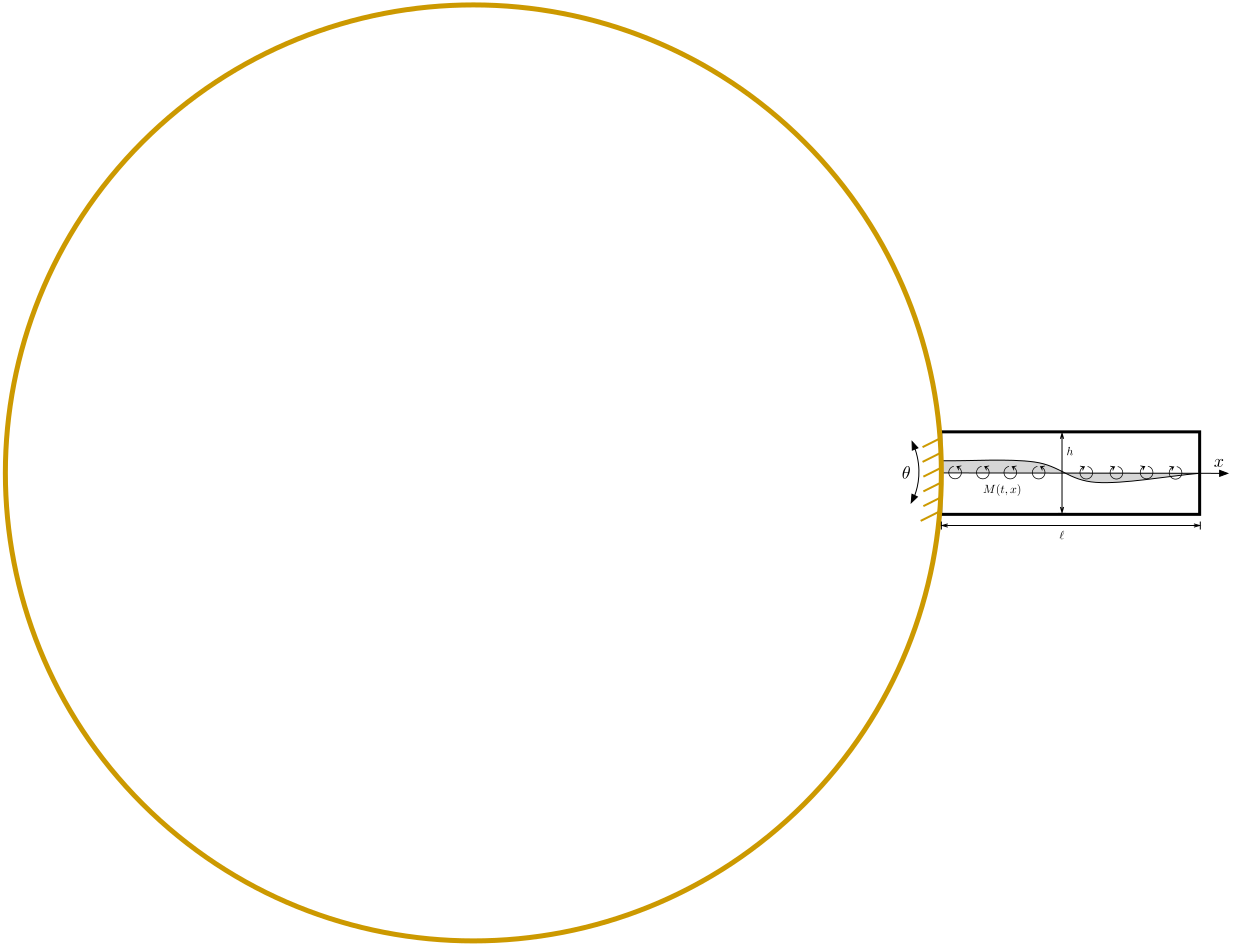
\includegraphics[width=\columnwidth,trim=12.46in 5.3in 0in 5.44in,clip=true]{../ch7/figures/varbeam-c-ut-2}
\caption{Continuously distributed internal moment on a uniform thickness array.}\label{fig:ch7:varbeam-c-ut}
\end{subfigure}
\hspace{0.005\columnwidth}
\begin{subfigure}[b]{0.49\columnwidth}
\centering 
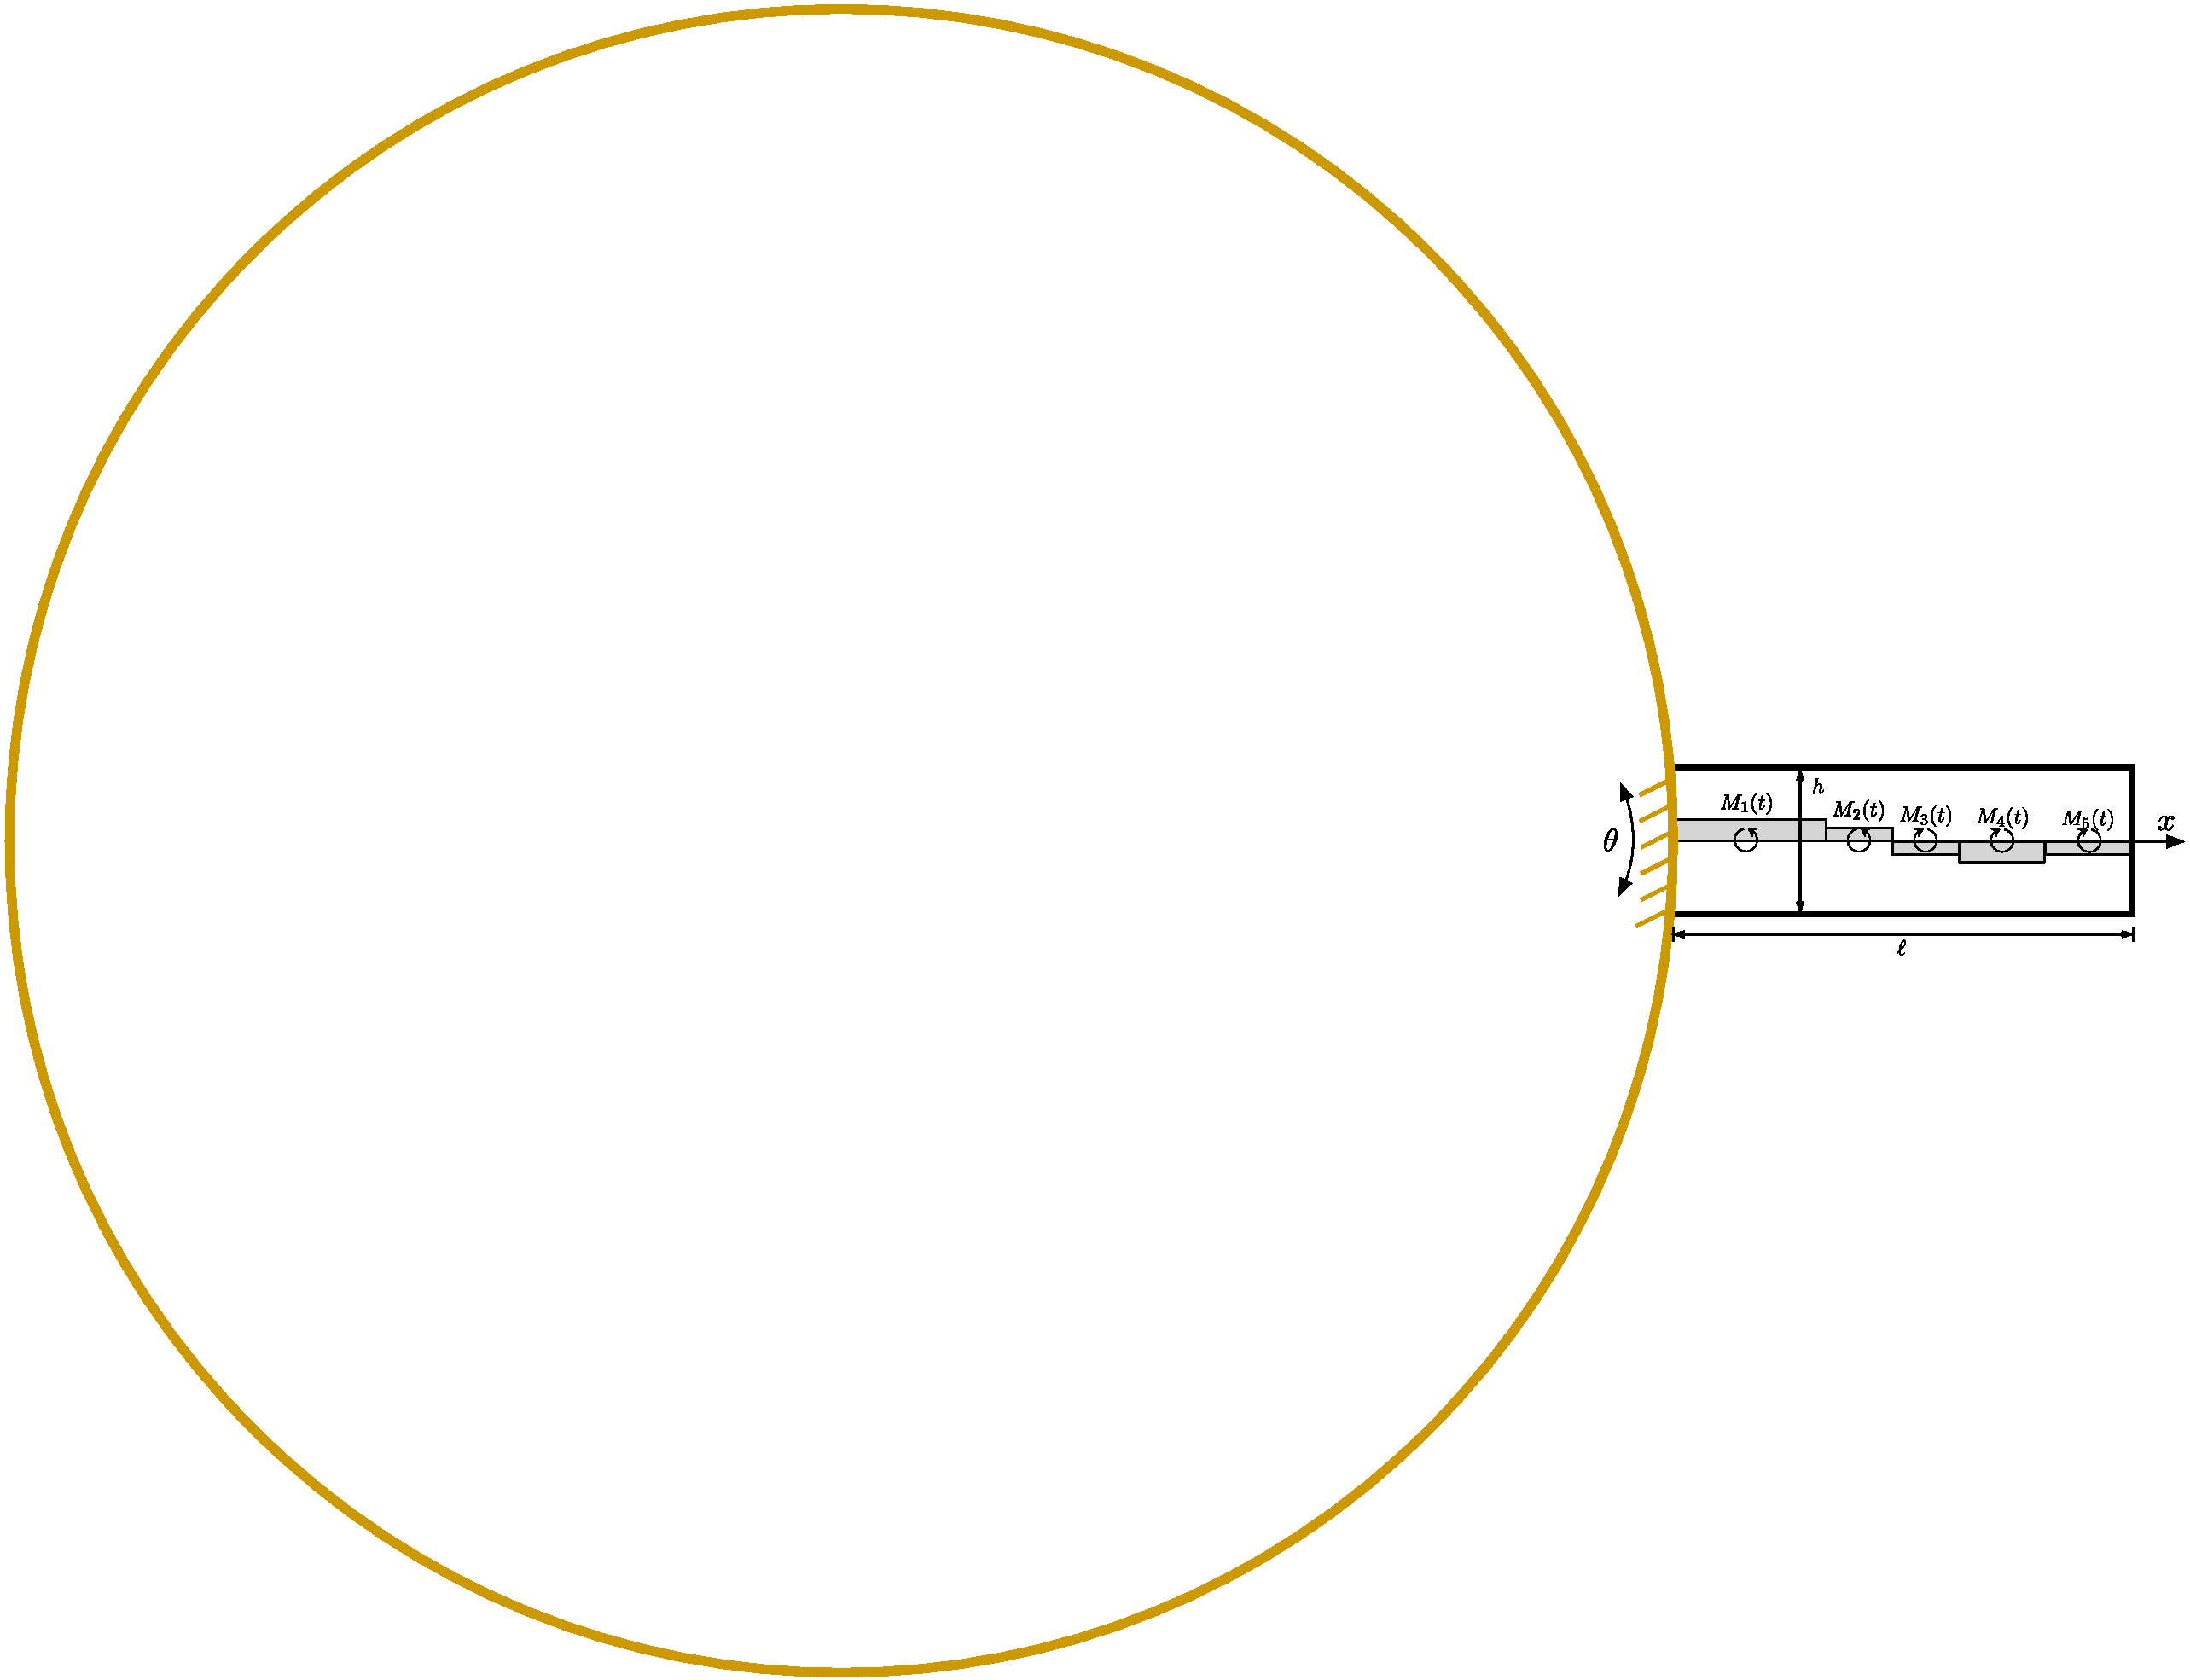
\includegraphics[width=\columnwidth,trim=12.46in 5.3in 0in 5.44in,clip=true]{../ch7/figures/varbeam-d-ut-2}
\caption{Piecewise constant distributed internal moment on a uniform thickness array.}\label{fig:ch7:varbeam-d-ut}
\end{subfigure}%

\begin{subfigure}[b]{0.52\columnwidth}
\centering 
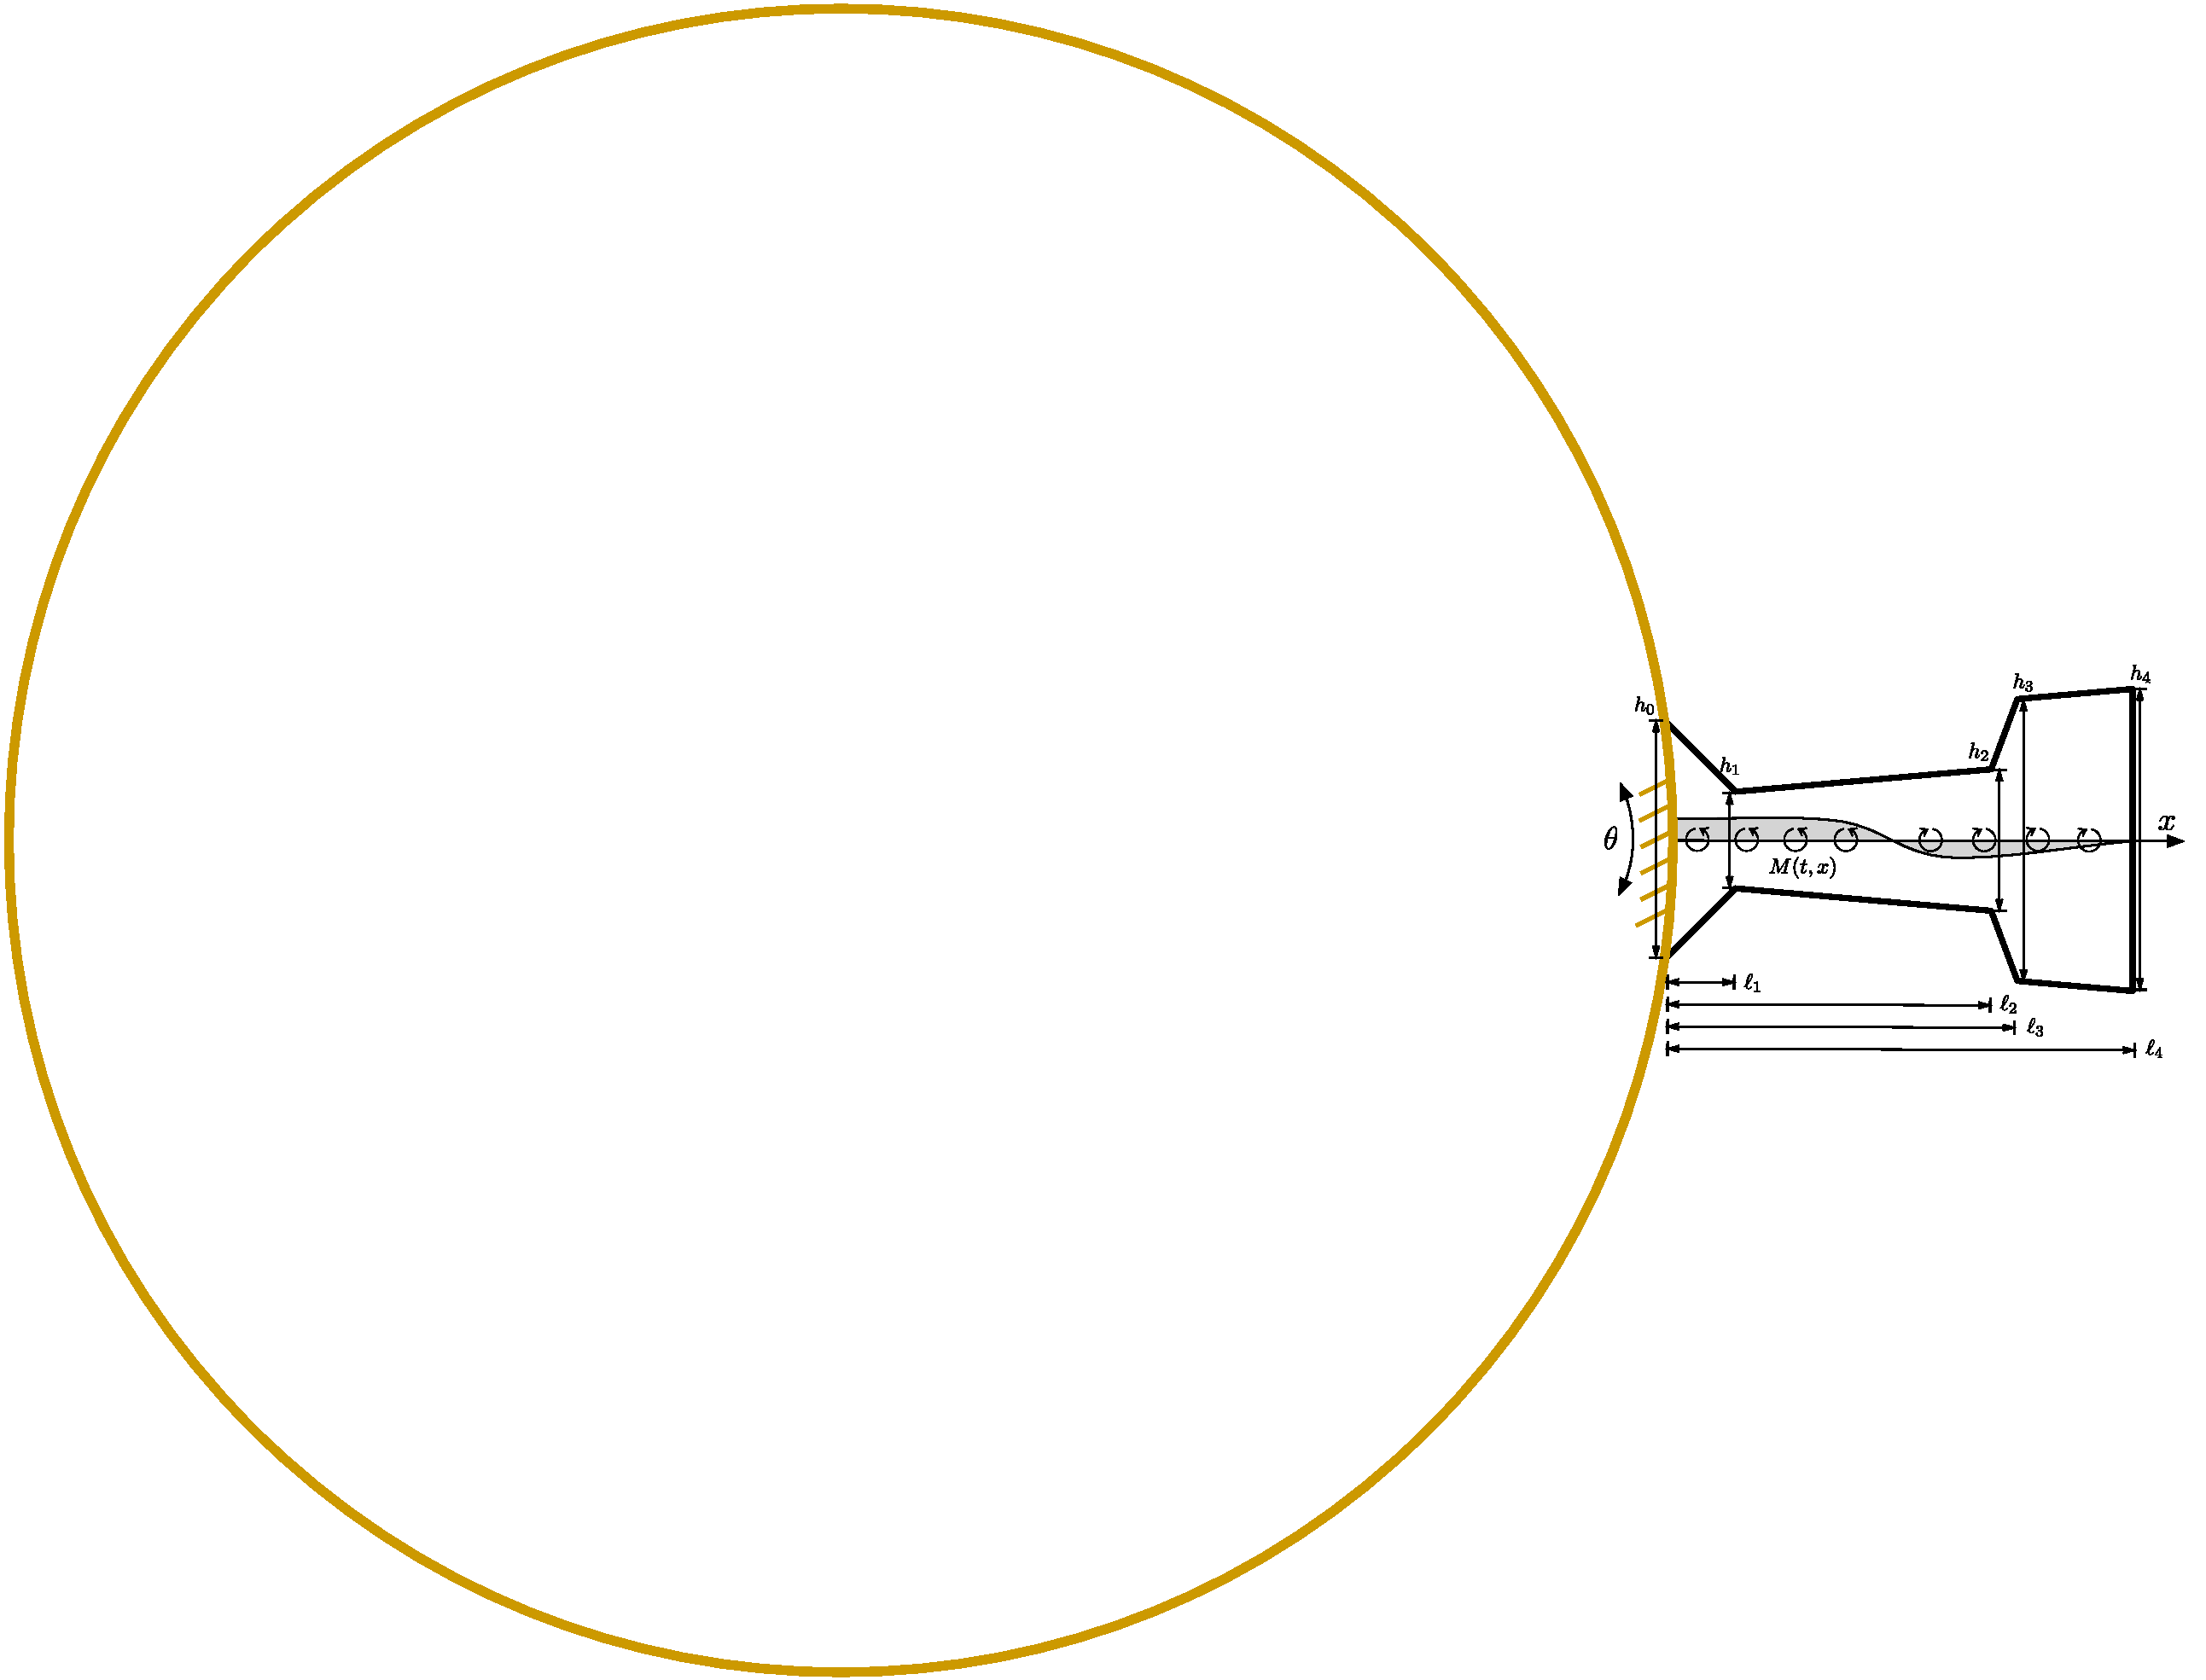
\includegraphics[width=\columnwidth,trim=12.46in 4.8in 0in 5.1in,clip=true]{../ch7/figures/varbeam-c-vt-2}
\caption{Piecewise linear distributed array thickness.}\label{fig:ch7:varbeam-c-vt}
\end{subfigure}%

\caption{Illustrations of various design representations for internally actuated array design problems for pointing. \label{fig:ch7:varbeam}}
\end{figure}

\subsubsection{Galerkin Formulation}

To approximate numerically the PDE in Eqn.~(\ref{eq:ch7:PDEdynamics_linear}), we use a Galerkin formulation~\cite{Junkins1993a, Paranjape2012a, Paranjape2013a}. A linear combination of approximating functions is used to represent the array dynamic state~\cite{Junkins1993a} and distributed moment. These functions are chosen such that they satisfy the boundary conditions of the array, i.e.,~the fixed-free condition. The $j$th approximating functions used for spatially distributed deflection and moment representations, respectively, are defined as~\cite{Junkins1993a}:
\begin{align}
\phi_{j}(x) = 1- \cos \left(\frac{j \pi x}{\ell} \right) +\frac{1}{2}(-1)^{j+1} \left(\frac{j \pi x}{\ell} \right)^{2}, \qquad 
\gamma_{j} (x) = \phi_{j}(x)+x^{j}+1 \label{eq:ch7:modes}
\end{align}

\noindent The array deflection and distributed moment are then approximated as:
\begin{align}
\xi(x,t) = \gls{phi}\tran \gls{eta}, \qquad M(x,t) = \gls{gamma}\tran \gls{q}
\end{align}

\noindent For the co-design studies here, four approximating functions are used. This approximation parameterizes the control as a spatially-varying distributed moment, but the actual control input on a piezoelectric segment is normally a uniform voltage \cite{Moheimani2006a}. Comparing both of these representations in Figs.~\ref{fig:ch7:varbeam-c-ut} and \ref{fig:ch7:varbeam-d-ut}, we may think of the spatially-varying distributed moment as the limiting case of the piecewise uniform moment (segment length approaching zero). The applicability of this approximation to a real implementable physical system will be discussed in Sec.~\ref{sec:ch7:placement}.

A system of ODEs that approximate the PDE given above is derived~\cite{Nakka2016a} by minimizing weighted residual of the $\xi$ dynamics. Using the above formulation and defining additional matrices we obtain:
\begin{gather}
\begin{aligned}
\bm{[M_{g}]} \begin{bmatrix} \ddot{\theta} \\ \ddot{\bm{\eta}} \end{bmatrix} +  \begin{bmatrix} 0 \\  2\bm{[e]}(\bm{\eta} +\mu \dot{\bm{\eta}}) \end{bmatrix} = \begin{bmatrix} d \\ \int_{0}^{\ell} 2 \bm{\phi} M^{''} dx \end{bmatrix}
\end{aligned}\label{eq:ch7:EL_system} \\
\begin{gathered}
\text{where:} \qquad \bm{[M_{g}]} = \begin{bmatrix} J_{\theta} + 2\int_{0}^{\ell} m_{R}\left(x+r\right)^2 dx  & 2 \bm{[B]} \\ 2 \bm{[B]}\tran & 2\bm{[A]} \end{bmatrix} \\
 \bm{[A]} = \int_{0}^{\ell} m_{R}\bm{\phi} \bm{\phi}\tran dx, \qquad  \bm{[B]}= \int_{0}^{\ell} m_{R}(x+r) \bm{\phi}\tran dx,
\qquad \bm{[e]} =\int_{0}^{\ell} \bm{\phi} \left(EI\bm{\phi}^{''{\mkern-1.5mu\mathsf{T}}} \right)^{''} dx
\end{gathered} \notag
\end{gather}

\subsubsection{Structural Model of Composite Array \label{sec:ch7:structural}}

The structural geometry of the array is also designed with the distributed moment. In this work, the length of the array and the distributed thickness are optimized. The spatially varying array thickness design is represented using piecewise linear segments. The length of the array is divided into multiple segments as shown in Fig.~\ref{fig:ch7:varbeam-c-vt}. Segment lengths and slopes can be changed. The distributed array thickness design is parameterized using the absolute locations of the segment boundaries (quantified by the vector \gls{lengths}), and the thickness at the segment boundaries (quantified by the vector \gls{heights}). On the segment $j$, the thickness varies linearly with respect to $x$ as follows:
\begin{align}
\begin{aligned}
h_j(x)=(h_{j+1}-h_{j})\frac{x-\ell_{j}}{\ell_{j+1}-\ell_{j}}+h_{j}, \qquad x \in [\ell_j,\ell_{j+1}]
\end{aligned} \label{eq:ch7:thickness}
\end{align}

The array is laminated with a layer of piezoelectric material on the top surface which acts as an actuator and has the same width as the beam. It is also assumed that the entire top surface of the array is covered with a piezoelectric layer of constant thickness $h_{\glsfirst{materialarray}}$. The neutral axis of the composite beam is not at the center due to the inhomogeneous structural properties. Consider the cross section of the composite beam shown in Fig.~\ref{fig:ch7:compositebeam}. The distance from the neutral axis and the top surface of the array with piezoelectric material is \gls{axis}. The thickness of the base array and the piezoelectric layer are $h_{\glsfirst{basearray}}(x)$ and $h_{e}$, respectively. Note that $h_{b}(x)$ can vary spatially. The neutral axis location $h_n$, for each position $0\leq x \leq \ell$, can be obtained by balancing the forces across the cross section and solving for $h_n$:
\begin{align}
h_n = \frac{0.5 E_{e} h_{e}^{2} + E_{b} h_{b} \left(0.5 h_{b} + h_{e}\right)}{E_{e}h_{e}+E_{b}h_{b}}
\end{align}

\begin{figure}[t]
\centering
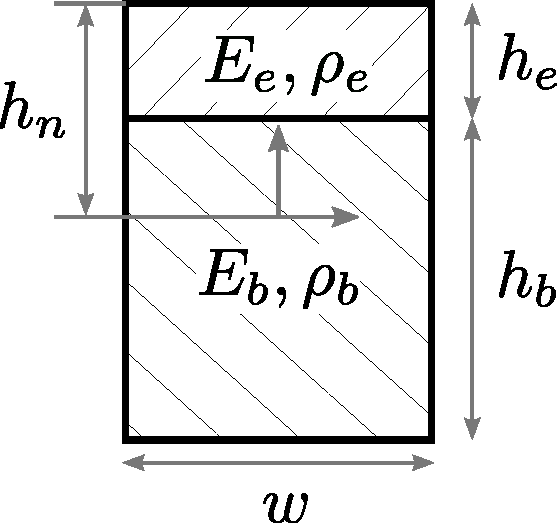
\includegraphics[height=1.4in]{../ch7/figures/BeamCrossSection2}
\caption{Cross section of the actuated array, modeled as a composite beam.} \label{fig:ch7:compositebeam}
\end{figure} 

\noindent The area moments of inertia of the array, $I_{b}$, and the piezoelectric layer, $I_{e}$, about the neutral axis are:
\begin{align}
I_{b} = \frac{w h_{b}^{3}}{12}  + w h_{b} \left(h_{e} + 0.5 h_{b} - h_n \right)^{2}, \qquad I_{e} = \frac{w h_{e}^{3}}{12} + w h_{e} \left(h_n  - 0.5 h_{e}\right)^{2} 
\end{align}

\noindent The total array rigidity is given by:
\begin{align}
EI = E_{b}I_{b} + E_{e}I_{e}
\end{align}

\noindent The mass per unit length of the composite array is $m_{R}(x) = m_{Rb}(x) + m_{Re}(x)$, where $m_{Rb}(x)$ and $m_{Re}(x)$ are the mass per unit length of the base array and the piezoelectric material, respectively. The application of a voltage \gls{voltage} across the piezoelectric layer induces a moment $M$. This moment, due to only internal actuation, can be calculated by applying force balance across the cross section of the composite array~\cite{Nakka2016a}:
\begin{align}
M(x,t) &= \gls{ccoefficient} V(x,t), \label{actuator_response}\\
\text{where: } c(x) &= \frac{d_{31} E_{b}^{2} w h_{b}^3 E_{e}  h_{b} (h_{b}+h_{e}) }{2 (E_{b}^2h_{b}^4 + 4E_{b}E_{e}h_{b}^3h_{e} + 6E_{b}E_{e}h_{b}^2h_{e}^2 + 4E_{b}E_{e}h_{b}h_{e}^3 + E_{e}^2h_{e}^4)} \notag
\end{align}

\noindent and $d_{31}$ is the ratio of the strain and the electric field applied across the piezoelectric layer when all the external forces are held constant~\cite{Moheimani2006a}. Observe that the moment is proportional to the applied voltage.

\subsection{Pseudo-Rigid Body Dynamic Model}

A PRBDM was developed for the spacecraft system for the purpose of performing additional numerical studies that complement those based on the PDE model, including studies that yield qualitative insights that are difficult to obtain via the more sophisticated PDE model. The flexible solar arrays were modeled both with single and multi-link approximations. The single link model is presented here, where each array is modeled as a single rigid link connected to the spacecraft body via a revolute joint and a torsional spring (see Fig.~\ref{fig:ch7:prbdm}). This is a lumped compliance approximation of the distributed compliance of the actual solar array. However, these models only describe the behavior at a component level rather than the specific point-to-point variations, while Euler-Bernoulli beam in Sec.~\ref{sec:ch7:beam} does capture these variations.

Applying the Euler-Lagrange equation to the system in Fig.~\ref{fig:ch7:prbdm} we arrive at the following equations of motion:
\refstepcounter{equation}
\begin{gather}
\bm{M}_{\glsfirst{pr}} \begin{bmatrix}
\ddot{\theta} \\ \ddot{\delta}
\end{bmatrix}  + \bm{B}_{\text{PR}} \begin{bmatrix}
\dot{\theta} \\ \dot{\delta}
\end{bmatrix} + \bm{K}_{\text{PR}} \begin{bmatrix}
{\theta} \\ {\gls{delta}}
\end{bmatrix} = \bm{\tau} \tag{\theequation}  \\
\begin{gathered}
\text{where:} \qquad \bm{M}_{\text{PR}} = \begin{bmatrix}
J_\theta + 2J_{\glsfirst{notdelta}} + 2 m r^2 + \frac{1}{2}m\ell^2 + 2 \ell m r \cos(\delta) & 2J_\delta + mr\ell\cos(\delta) + \frac{1}{2}m\ell^2 \\
2J_\delta + mr\ell\cos(\delta) + \frac{1}{2}m\ell^2 & 2J_\delta + \frac{1}{2}m\ell^2
\end{bmatrix}  \\
\bm{B}_{\text{PR}} = \begin{bmatrix}
-2\ell m r \dot{\delta} \sin(\delta) & - \ell m r \dot{\delta}\sin(\delta) \\
\ell m r \dot{\theta} \sin(\delta) & 2b
\end{bmatrix}, \qquad \bm{K}_{\text{PR}} = \begin{bmatrix}
0 & 0 \\ 0 & 2k
\end{bmatrix}, \qquad
\bm{\tau} = \begin{bmatrix} d \\ 2M \end{bmatrix}
\notag \\
\gls{mass} = \gls{density} \ell w h, \qquad J_{\delta} = \frac{1}{12}m \left(\ell^2 + h^2\right)
\end{gathered} \notag
\end{gather}

\noindent and where \gls{spring} is the torsional spring stiffness and \gls{damper} is the damping constant at the revolute joints. Solving the eigenvalue problem ($\bm{M}_{\text{PR}}^{-1}\bm{K}_{\text{PR}} = \gls{omega}^2$) gives the natural frequencies of the system: \refstepcounter{equation}
\begin{subequations}
\small
\begin{align}
\omega_1^2 &= 0 \\
\omega_2^2 &= k \frac{2 m \ell^2 + 8 m \ell r \cos\left(\delta\right) + 8 m r^2 + 4 J_{\theta} + 8 J_{\delta}}{ - 2\ell^2 m^2 r^2 {\cos\left(\delta\right)}^2 + 2 \ell^2 m^2 r^2 + J_{\theta} \ell^2 m + 8 J_{\delta} m r^2 + 4 J_{\theta} J_{\delta}} = \frac{k}{J_{\text{eff}}\left(\delta,\ell,h,w\right)} 
\end{align}
\end{subequations}

\noindent One of the eigenfrequencies is zero since the system permits a rigid body mode. The two mode shapes are:
\begin{align}
\gls{modes} = \begin{bmatrix}
\bm{\psi}_1 & \bm{\psi}_2 
\end{bmatrix} = \begin{bmatrix}
1 & -\frac{m \ell^2 + 2 m r \ell \cos(\delta)  + 4 J_{\delta}}{m \ell^2 + 4 m r \ell \cos(\delta) + 4 m r^2 + 2 J_{\theta} + 4 J_{\delta}} \\ 0 & 1
\end{bmatrix}
\end{align}

\noindent We note that the nonrigid mode eigenfrequency ($\omega_2$) and eigenvector ($\bm{\psi}_2$) are not constant but depend on the path of the array. The total angular momentum of the system is:
\begin{align}
\hspace{-0.5ex}\gls{momentum}= \left( \frac{1}{2} \ell^2 m +  2 \ell m r \cos(\delta) + 2mr^2 + J_\theta + 2J_\delta  \right) \dot{\theta} + \left( \frac{1}{2} \ell^2 m + \ell m r \cos(\delta) + 2J_\delta \right)  \dot{\delta} \label{eq:ch7:momentum}
\end{align}

\noindent Since internal moments cannot change the total angular momentum of the system, the only mode that is present in the absence of external moments is the momentum conserving mode $\bm{\psi}_2$.

\section{Co-Design Problem Formulation \label{sec:ch7:formulation}}

The objective of the co-design study is to provide insights into how the actively-controlled solar array should be designed to optimize the performance in terms of attitude slewing and jitter reduction. A balanced co-design approach is utilized where physical-system (geometric specification of the solar array) and control-system (open-loop voltage trajectories) design are considered in an equally comprehensive manner \cite{Allison2014b}. A general simultaneous co-design formulation (with a fixed time horizon) is in Prob.~(\ref{eq:simprob}).
Here the physical system design $\gls{x}_{\glsfoo[noindex]{plant}}$ is parameterized by $\bm{h}$ and $\bm{\ell}$ with eight distinct linear segments. The control system design variable is defined here as $\bm{x}_{\glsfoo[noindex]{control}} := \bm{q}(t)$; these control trajectories are used to compute $M(x,t)$ and $V(x,t)$.

The spacecraft control task is divided into two consecutive phases; \gls{middle} is the time duration of the first phase. The first phase (slewing) concentrates on rotating the bus from an initial angular displacement $\theta(t_{\glsfoo[noindex]{initial}})$ back to $\theta = 0$ at time $t_m$. In the second phase (pointing) the bus is held inertially fixed for precision pointing. Any vibrations generated during slewing must be damped out during the pointing phase. The objective function is to maximize the slewing angle, demonstrating the maximum capability of the SASA attitude control system:\refstepcounter{equation}
\begin{align}
\gls{objective} = -\theta(t_0) \tag{\theequation a} \label{eq:ch7:obj}
\end{align}

\noindent where $t \in [t_0,t_{\glsfoo[noindex]{final}}] = [0 \text{ s},t_m+1\text{ s}]$ and $t_m$ is solved at various values between 0.12 s and 4 s. This parametric sweep on $t_m$ helps quantify the tradeoff between the competing objectives of slew angle maximization and slew time minimization. The dynamic constraint uses the linear ODE defined in Eqn.~(\ref{eq:ch7:EL_system}) with 4 approximating functions. The physical parameters for the bus, array, and piezoelectric layer are shown in Table~\ref{tb:ch7:parameters}. A disturbance moment $d(t)$ on the bus is present during the slewing and pointing phases. It consists of a jitter component (e.g.,~vibrations similar to those that arise from moving parts such as pumps) and a bias component (e.g.,~due to solar radiation pressure, atmospheric drag):
\begin{align}
d(t) = 10^{-4} \text{ Nm} + 2\times 10^{-3}\sin(50t)  \text{ Nm}  \tag{\theequation b} \label{eq:ch7:disturbance}
\end{align}

\begin{table}[t]
\centering
\begin{subfigure}[t]{0.5\textwidth}
    \centering
    \caption{Bus parameters.}
	\begin{tabular}{cl}
	\hline \hline
	Parameter & Value \\
	\hline
	$J_{\theta}$ & 372.49 kg m$^2$  \\
	$r$ & 1.02 m  \\
	\hline \hline
	\end{tabular}
\end{subfigure}%
\begin{subfigure}[t]{0.5\textwidth}
    \centering
	\caption{Array and piezoelectric material parameters.}
	\begin{tabular}{cl}
	\hline \hline
	Parameter & Value \\
	\hline
	$\ell_{\text{nominal}}$ & 1.575 m \\
	$h_{\text{nominal}}$ & 0.018 m \\
	$w_{\text{nominal}}$ & 1.862 m \\
	$h_p$ & $2 \times 10^{-4}$ m \\
	$E_b$ & 1.57 GPa \\
	$\rho_b$ & 332.03 kg/m$^3$ \\
	$E_p$ & 62 GPa \\
	$\rho_p$ & 7800 kg/m$^3$ \\
	$\mu$ & $10^{-4}$ s \\
	\hline \hline
	\end{tabular}
\end{subfigure}%

\caption{Problem physical parameters.} \label{tb:ch7:parameters}

\end{table}

\noindent The initial configuration is stationary with an initial bus orientation $\theta_0=\theta(t_0)\neq 0$. The initial states\footnote{The states $\bm{\xi}$ include the deflection $\xi$ of the array in Fig.~\ref{fig:ch7:coordinate} through $\bm{\eta}$.} are:
\begin{align}
\gls{states}(t_0) =
\begin{bmatrix}
\theta(t_0) \\ \dot{\theta}(t_0) \\  \bm{\eta}(t_0) \\ \dot{\bm{\eta}}(t_0)
\end{bmatrix} =
\begin{bmatrix}
\theta_0 \\ 0 \\ \bm{0} \\ \bm{0}
\end{bmatrix} \tag{\theequation c}  \label{eq:ch7:init_condition}
\end{align}

\noindent The bus angle and angular rate are constrained to 0 during the pointing phase. This simultaneously meets the pointing task and eliminates jitter if a feasible solution is found:
\begin{align}
\abs{\theta(t)} &= 0, \qquad t \in [t_m,t_{f}] \tag{\theequation d} \label{eq:ch7:theta_path} \\
\abs{\dot{\theta}(t)} &= 0, \qquad t \in [t_m,t_{f}] \tag{\theequation e} \label{eq:ch7:dtheta_path}
\end{align}

\noindent Numerical experiments indicate these constraints can be satisfied in all but very unusual cases. PEMA actuation magnitude is constrained to satisfy maximum voltage restrictions:
\begin{align}
\abs{V(x,t)} = \abs*{\frac{M(x,t)}{c(x)}} \leq 300 \text{ V} \tag{\theequation f} \label{eq:ch7:voltage}
\end{align}

\noindent The array surface strain is constrained to be less than 0.1\% to maintain structural integrity:
\begin{align}
\abs{\gls{strain}} = \abs*{\left( h_{b}(x) + h_e - h_n(x) \right) \xi^{''}(t) } \leq 10^{-3} \tag{\theequation g} \label{eq:strain}
\end{align}

\noindent Traditional silicon-based solar cells can withstand strain levels on the order of 0.1\% \cite{Lindmayer1977a}. However, recent advances allow the manufacturing of flexible solar cells that can achieve strain levels on the order of 10\% \cite{Lee2011a}, as well as fiber-shaped solar cells that can be woven into textiles \cite{Qiu2016a}.

The total array length, linear array segment lengths, and array thickness values have manufacturing and operational constraints:
\begin{gather}
\begin{gathered}
0.5 \text{ m} \leq \ell_{n} \leq 2.5 \text{ m}  \\
0.05 \text{ m} \leq \ell_{i+1} - \ell_{i} \leq 1 \text{ m}  \\
0.009 \text{ m} \leq h_{i} \leq 0.055 \text{ m} 
\end{gathered} \qquad i = 0, 1, \dots, n \tag{\theequation h} \label{eq:geometrybounds}
\end{gather}

\noindent The array volume is constrained to be less than the nominal value in order to avoid increasing the payload mass and delivery costs. This is proportional to the array structure cross-sectional area:
\begin{align}
\sum_{i=1}^{n} \frac{w}{2}(h_{i-1}+h_{i})(\ell_{i}-\ell_{i-1}) \leq 0.054 \text{ m}^3 \tag{\theequation i} \label{eq:ch7:volume_con}
\end{align}

\noindent Array planform area is constrained to the nominal value to maintain the same level of power generation:
\begin{align}
\ell_{n}w = 2.932 \text{ m}^2 \tag{\theequation j} \label{eq:ch7:area_con}
\end{align}

\noindent Direct orientation of the solar arrays towards the sun requires the attitude rotation axis to be normal to the sun-spacecraft vector. Solar power generation is a function of array area and orientation (and other factors). The planform area constraint is intended to be large enough to ensure adequate overall power generation even when arrays are not oriented directly toward the sun. A more sophisticated and accurate approach would model power generation directly across a range of maneuvers and insolation conditions. An investigation of the tradeoff between power generation and attitude control is a topic for future work.

This completes the exposition of the co-design problem formulation; objective and constraint functions are summarized in Table~\ref{tb:ch7:codesign_summary}. Note that some optimization variables (states and controls) are linear while other variables (plant parameters) are nonlinear in the co-design formulation. A traditional approach to solve this type of problems is to use nested co-design \cite{Allison2014b,  Fathy2001a, Herber2017b}. 
This approach consists of an outer-loop that finds the optimal plant parameters, while the inner-loop finds the optimal states and controls histories for each point in the plant parameter space sampled by the outer-loop. In this way, the inner-loop can return the cost of a particular plant design to the outer-loop. Since the the optimal control problem in the inner-loop is linear, it can be formulated and solved as a \glsfirst{LP} using a direct transcription method \cite{Enright1992a, Betts2010a, Biegler2010a, Herber2014a}. Direct transcription has been used traditionally in trajectory optimization \cite{Chilan2013a, Betts2010a, Morgan2014a}. The custom transcription code in Chapter~\ref{ch:5} was used to transform the infinite dimensional optimal control problem into a finite dimensional optimization problem.
The structure-based description is in the following section.

A feasible solution for the inner-loop problem is globally-optimal because it is formulated as an LP program. However, the nonlinear dependencies on the plant parameters in the outer-loop require special attention to ensure that the global optimum is found. The outer loop is implemented using \xprog{Matlab} \xprog{patternsearch} \cite{matlab-patternsearch}, while the inner-loop is implemented using \xprog{Matlab} \xprog{quadprog} \cite{matlab-quadprog}. \xprog{Matlab} \xprog{patternsearch} was configured to use complete search (Latin hypercube sampling) and polling options to help find the global solution.

In an earlier version of this work \cite{Chilan2016a}, the nonlinear dynamics were directly used. Therefore, the methods from Chapter~\ref{ch:5} were not applicable. A nonlinear dynamic optimization software package was instead used to solve the problem using the simultaneous co-design method from Chapter~\ref{ch:3}.
However, there were a number of problems with this strategy. The computation time was extremely large, making it impossible to perform tests on a variety of starting points or problem parameters, so there was less confidence in the global optimality of the solution and less information gained. One reason for this large computation time was the fact that the plant-dependent quantities needed to be updated frequently when the simultaneous approach was used. The nested approach, on the other hand, typically tests a smaller number of candidate plant designs.
Additionally, the control was not guaranteed to be the global optimum, as is the case here.

The results for a number of minor variations of this formulation will be discussed next after a short study on the fundamental limits of a slewing maneuver with SASA utilizing a reduced form of this co-design formulation and the PRBDM model. 

\begin{table}
\caption{Summary of co-design problem formulation. \label{tb:ch7:codesign_summary}}
\centering
\begin{tabular}{rccccc}
\hline \hline
& & \multicolumn{3}{c}{Linear w.r.t.} & \\
Name & Eqn.~\# & $\bm{\xi}$ & $ \bm{x_c}$ & $\bm{x_p}$ & Level \\
\hline
Max. Slew Amount & Eqn.~(\ref{eq:ch7:obj}) & Yes & & & Both \\
Dynamics & Eqn.~(\ref{eq:ch7:EL_system}) \& Eqn.~(\ref{eq:ch7:disturbance}) & Yes & Yes & No & Inner \\
Initial Conditions & Eqn.~(\ref{eq:ch7:init_condition}) & Yes & & & Inner \\
Pointing & Eqn.~(\ref{eq:ch7:theta_path}) \& Eqn.~(\ref{eq:ch7:dtheta_path}) & Yes & & & Inner \\
Voltage Limits & Eqn.~(\ref{eq:ch7:voltage}) & & Yes &  No & Inner \\
Strain Limits & Eqn.~(\ref{eq:strain}) & Yes & & No & Inner  \\
Geometry Bounds & Eqn.~(\ref{eq:geometrybounds}) & & & Yes & Outer \\
Array Volume & Eqn.~(\ref{eq:ch7:volume_con}) & &  & No & Outer \\
Planform Area & Eqn.~(\ref{eq:ch7:area_con}) & & & No & Outer \\
\hline \hline
\end{tabular}
\end{table}

\subsection{Inner-Loop Structure-Based Description}

Here we present the structure-based description for the \lqdo{} problem.
The approach from Chapter~\ref{ch:5} is utilized twice, once for each phase.
Then the LPs created for each phase are linked with linear continuity constraints (see Sec.~\ref{sec:ch5:multipleinterval}) for the states.

The maximum slew objective in Eqn.~(\ref{eq:ch7:obj}) is implemented with a single Mayer term:%
\begin{gather}
\mathcal{M}\xind{1}.\xvar{left} = 0, \quad \mathcal{M}\xind{1}.\xvar{right} = 4, \quad \mathcal{M}\xind{1}.\xvar{matrix} = \begin{bmatrix}-1 & \bm{0} \end{bmatrix} 
\end{gather}

\noindent The initial conditions in Eqn.~(\ref{eq:ch7:init_condition}) are implemented with simple bounds in the first phase:%
\begin{subequations}%
\begin{gather}%
\mathcal{UB}\xind{\cdot}.\xvar{right} = 2, \quad \mathcal{UB}\xind{\cdot}.\xvar{matrix} = \begin{bmatrix} \infty & \bm{0} \end{bmatrix}\tran \\
\mathcal{LB}\xind{\cdot}.\xvar{right} = 2, \quad \mathcal{LB}\xind{\cdot}.\xvar{matrix} = \begin{bmatrix} -\infty & \bm{0} \end{bmatrix}\tran
\end{gather}
\end{subequations}

\noindent The bus angle and angular rate equality constraints in Eqns.~(\ref{eq:ch7:theta_path})--(\ref{eq:ch7:dtheta_path}) are implemented with simple upper and lower bounds only in the second phase:%
\begin{subequations}%
\begin{gather}%
\mathcal{UB}\xind{\cdot}.\xvar{right} = 2, \quad \mathcal{UB}\xind{\cdot}.\xvar{matrix} = \begin{bmatrix} 0 & 0 & \bm{\infty} \end{bmatrix}\tran \\
\mathcal{LB}\xind{\cdot}.\xvar{right} = 2, \quad \mathcal{UB}\xind{\cdot}.\xvar{matrix} = \begin{bmatrix} 0 & 0 & -\bm{\infty} \end{bmatrix}\tran
\end{gather}
\end{subequations}

\noindent The absolute value limits on the voltage in Eqn.~(\ref{eq:ch7:voltage}) are implemented with linear inequality at each test point $x_i$ in both phases:%
\begin{subequations}%
\begin{gather}%
\mathcal{Z}\xind{\cdot}.\xvar{linear}\xind{1}.\xvar{right} = 1, \quad  \mathcal{Z}\xind{\cdot}.\xvar{linear}\xind{1}.\xvar{matrix} = \bm{\gamma}(x_i), \quad \mathcal{Z}\xind{\cdot}.\xvar{b} = V_{\glsfoo[noindex]{max}} c(x_i) \\
\mathcal{Z}\xind{\cdot}.\xvar{linear}\xind{1}.\xvar{right} = 1, \quad  \mathcal{Z}\xind{\cdot}.\xvar{linear}\xind{1}.\xvar{matrix} = -\bm{\gamma}(x_i), \quad  \mathcal{Z}\xind{\cdot}.\xvar{b} = V_{\max} c(x_i)
\end{gather}
\end{subequations}

\noindent The absolute value limits on the strain in Eqn.~(\ref{eq:strain}) are implemented with linear inequality at each test point $x_i$ in both phases:%
\begin{subequations}%
\begin{gather}%
Z = \begin{bmatrix} 0 & 0 & (h_b(x_i) + h_e - h_n(x_i)) \bm{\phi}''(x_i) & \bm{0} \end{bmatrix}\tran \\
\mathcal{Z}\xind{\cdot}.\xvar{linear}\xind{1}.\xvar{right} = 2, \quad \mathcal{Z}\xind{\cdot}.\xvar{linear}\xind{1}.\xvar{matrix} = Z, \quad \mathcal{Z}\xind{\cdot}.\xvar{b} = \epsilon_{\max} \\
\mathcal{Z}\xind{\cdot}.\xvar{linear}\xind{1}.\xvar{right} = 2, \quad \mathcal{Z}\xind{\cdot}.\xvar{linear}\xind{1}.\xvar{matrix} = -Z, \quad \mathcal{Z}\xind{\cdot}.\xvar{b} = \epsilon_{\max}
\end{gather}
\end{subequations}

\section{Analytical and Numerical Results for SASA System\label{sec:ch7:results}}

\subsection{Maximum Slewing Bounds using the PRBDM \label{sec:ch7:prbdm_bounds}}

The momentum of the PRBDM system is given in Eqn.~(\ref{eq:ch7:momentum}), and it must be conserved if no external disturbance acts on the spacecraft ($d\equiv 0$). Assuming zero initial momentum, we can integrate the momentum equation to determine the relationship
between $\theta$ and $\delta$:
\begin{gather}
\begin{aligned}
0 &= \left( \frac{1}{2} \ell^2 m +  2 \ell m r \cos(\delta) + 2mr^2 + I_\theta + 2I_\delta  \right) \dot{\theta} + \left( \frac{1}{2} \ell^2 m + \ell m r \cos(\delta) + 2I_\delta \right)  \dot{\delta} \\
&:= I_1(\ell,h,w,\delta) \dot{\theta} + I_2(\ell,h,w,\delta) \dot{\delta} 
\end{aligned} \notag \\
\dot{\theta}  = - \frac{I_2(\delta,\cdot)}{I_1(\delta,\cdot)}   \dot{\delta} \notag \\
\theta(t_f) - \theta(t_0)= - \int_{t_0}^{t_f} \frac{I_2(\delta,\cdot)}{I_1(\delta,\cdot)}   \dot{\delta} dt 
\end{gather}

\noindent The question we are trying to answer requires an upper bound on $\abs{\theta(t_f) - \theta(t_0)}$. We can find a reasonable upper bound by determining the maximum value of the integrals. Recall that $m$ and $I_\delta$ are dependent on the geometric physical design variables. Since the geometric variables are positive and it is reasonable to assume $\cos(\delta) > 0$ (panel angle must be smaller than $\abs{\delta} < \pi/2$), then we see that the following difference is strictly positive: $I_1-I_2 = \ell m r \cos\left(\delta\right) + 2 m r^2 + I_{\theta} > 0$. Therefore, the effective inertia ratio, $\gls{Reff} := I_2/I_1$, must be between $0$ and $1$.

If $\abs{\delta(t)} \leq \delta_{\max}$ is small, then $R_{\mathrm{eff}}$ is nearly time-independent. Observe also that the effective inertia ratio is maximized when $\delta = 0$. Therefore, we will use this maximal value, denoted $R_{\mathrm{eff},\max}$, as a time-independent value to arrive at the following inequality:
\begin{align}
\abs{\theta(t_f) - \theta(t_0)} &\leq R_{\mathrm{eff},\max} \abs*{- \int_{t_0}^{t_f} \dot{\delta} dt} \notag \\
&\leq R_{\mathrm{eff},\max} \abs{\delta(t_0) - \delta(t_f)}
\end{align}

\noindent Assuming $\delta(t_0) = 0$, $\theta(t_f) = 0$, and that the prescribed bound on $\delta$ is hit at $t_f$, then we have:
\begin{align}
\abs{\theta_0} \leq R_{\mathrm{eff},\max} \delta_{\max} \leq \delta_{\max}
\end{align}

\noindent Therefore we expect the maximum change for the bus angle to be bounded above by the allowable change in panel angle using only internal actuation of the solar array. This implies that if only milli-radian deflections of the array are feasible, we can only achieve, at most, milli-radian changes in bus orientation. Additional novel solutions for SASA such as revolute joints that allow for large changes in the effective inertia ratio without violating conservation of momentum may extend this limit. 

A comparable $\delta_{\max}$ condition for a continuous array is a strain bound. If we want the largest value for $\delta$, analogously the strain will be at its maximum possible value at each point on the arrays. Using the constant thickness solar array in Fig.~\ref{fig:ch7:prbdm}, we can calculate this bound as $\delta_{\max} = (\ell/h) \epsilon_{\max}$. With this relationship, we can calculate the predicted maximum slewing bound. Two cases are shown in Table~\ref{tb:ch7:prbdm}: nominal geometry and maximum allowable value for $\ell$. The latter case achieves the maximum value of the slew bound since both $R_{\mathrm{eff,\max}}$ and $\delta_{\max}$ are maximized. We can also determine the actual maximum slew bound using the optimal control problem in Sec.~\ref{sec:ch7:formulation} (i.e.,~fixed geometry) without the voltage constraint. This result is also shown in Table~\ref{tb:ch7:prbdm} and indeed the bound is verified. The bound is not tight because the optimal voltage trajectories did not strain all of the array to the prescribed bound but only most of the array; thus, this assumption was only partially valid. 
In the next section, the study will consider the other design constraints and allow  piecewise-linear array thickness changes. The bounds in this section do not consider all the design constraints and therefore are only approximate indications of the maximum possible slewing performance.

\begin{table}
\caption{Summary of results for maximum slewing bounds using the PRBDM. \label{tb:ch7:prbdm}}
\centering
\begin{tabular}{rcccc}
\hline \hline
Study & $R_{\mathrm{eff},\max}$ & $R_{\mathrm{eff},\max} \delta_{\max}$ & & Actual \\ 
\hline
Nominal Geometry & 0.12 & 0.0108 rad (0.62$^\circ$) & $>$ & 0.0063 rad (0.36$^\circ$) \\  
Maximal $\ell$ & 0.22 & 0.0301 rad (1.73$^\circ$) & $>$ & 0.0176 rad (1.01$^\circ$) \\
\hline \hline
\end{tabular}
\end{table}

\subsection{Maximum Slewing Bounds using the Co-Design Problem Formulation}

In this section we study three variations of geometric design representation in the co-design problem introduced in Sec.~\ref{sec:ch7:formulation}. These are denoted \glsfirst{NG}, \glsfirst{VL}, and \glsfirst{PLS}. The geometric constraints for each case are summarized in Table~\ref{tb:ch7:parametric_study}. The NG case does not involve physical-system design since it is fixed and is only included in this study as a performance baseline. For the VL case, $\ell$ is the sole physical-system design variable (see Fig.~\ref{fig:ch7:varbeam-c-ut}). Finally, the PLS case varies total array length, segment lengths, and spatially-varying thickness to modify distributed geometric design of the array structure (see Fig.~\ref{fig:ch7:varbeam-c-vt}). The array volume (or mass) in the PLS case can be smaller than the nominal, whereas in the VL case, the volume is fixed to the nominal value of the NG case. Since the array planform area is constrained to a nominal value in each case, the array width is determined by the array length. Several values of the slewing time, $t_m$, between 0.12 s and 4 s were studied to investigate the relationship between slew time, the maximum slew angle, and corresponding optimal array designs. The final time of the simulation is given by $t_f=t_m+1$.

\begin{table}
\caption{Geometric constraints for the co-design problem variations. \label{tb:ch7:parametric_study}}
\centering
\begin{tabular}{rcccc}
\hline \hline
& \multicolumn{3}{c}{Array Property} \\
Variation & Length (m) & Thickness (m) & Volume (m$^3$) \\ 
\hline
NG & 1.575 & 0.018 & 0.054 \\
VL & $0.5 \leq \ell \leq 2.5$ & 0.018 & 0.054 \\
PLS & $0.5 \leq \ell \leq 2.5$ & $0.009 \leq h(x) \leq 0.055$ & $\leq 0.054$ \\
\hline \hline
\end{tabular}

\end{table}

\begin{figure}[t]
\centering
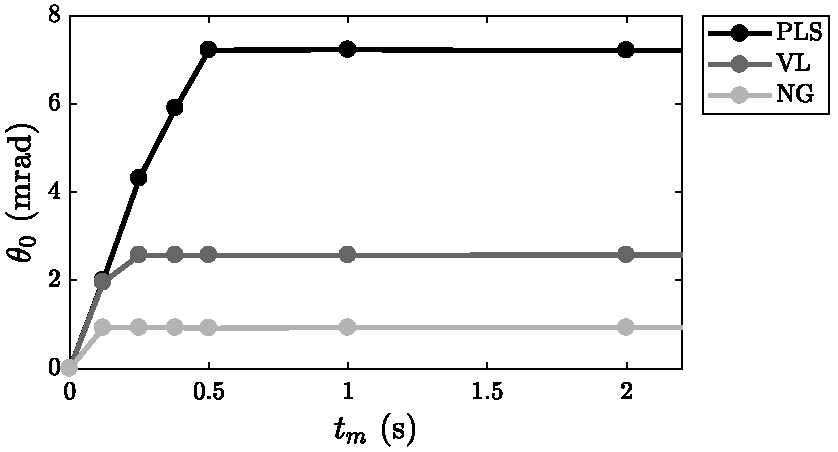
\includegraphics[width=0.6\columnwidth]{../ch7/figures/maxslew_parametric.pdf}
\caption{Parametric study of maximum slewing angle with respect to slewing time.}\label{fig:ch7:maxslew_parametric}
\end{figure}

The maximum slewing results for each of the three variations are summarized in Fig.~\ref{fig:ch7:maxslew_parametric}. As expected, the NG case achieved the smallest maximum slewing angle (0.9 mrad) for all the tested slewing times. This result indicates that the performance level desired may not be achievable through control design alone. Furthermore, the peak maximum achievable slewing angles for the VL and PLS cases (2.6 mrad and 7.2 mrad, respectively) are consistent with the results of Sec.~\ref{sec:ch7:prbdm_bounds}. The optimal array designs are shown in Fig.~\ref{fig:ch7:arrays_pls}. We observed that the optimal PLS geometries for slewing times $\geq 0.5$~s were similar. In addition, optimal VL designs for slewing times $\geq 0.25$~s are equal. The optimal trajectories for the bus angle and angular rate for the PLS and VL cases are shown in Fig.~\ref{fig:ch7:thetas}. These figures show that, through only internal actuation of the solar arrays, the slew maneuvers were performed and then the bus was held fixed (i.e.,~$\theta \equiv 0$ and $\dot{\theta} = 0$) for 1.0 sec all while managing jitter.

Note that for the VL case with slewing times of 0.25 sec and 1.0 sec, the bus angle trajectories are different, but the same slewing angle is achieved. Additional control-design-only problem formulations were conducted with $t_m$ up to 30 s and with the array design fixed as the optimal design from the 4 s slew time PLS solution. It was found that the maximum slewing angle remained equal to 7.2 mrad, indicating that a fundamental limit was reached. The limiting factor preventing larger slew angles here is the actuator voltage limit, as opposed to momentum limitations as detailed in Sec.~\ref{sec:ch7:prbdm_bounds}. Figure \ref{fig:ch7:voltage} illustrates that the actuator voltage is saturated during the pointing phase.

% maximum slewing angle
\begin{figure}[t]

    \begin{subfigure}[b]{\textwidth}
      \centering
      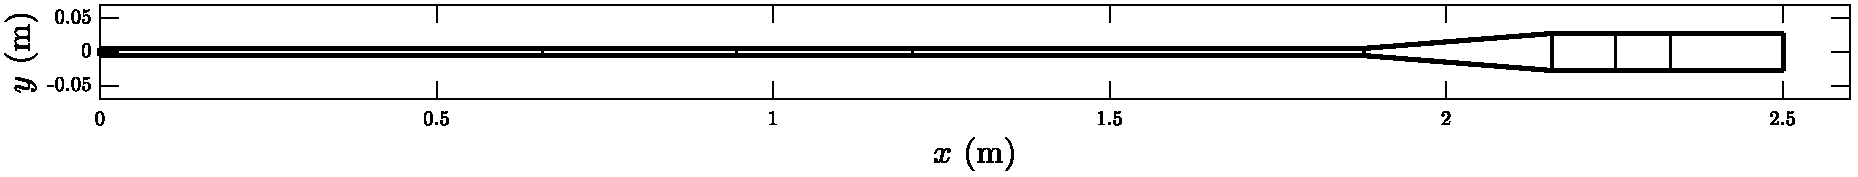
\includegraphics[width=\columnwidth]{../ch7/figures/UnscaledArray.pdf}
      \caption{Array design with maximal array inertia (drawn to scale).\label{fig:ch7:array_scale}}
    \end{subfigure}

    \begin{subfigure}[b]{\textwidth}
      \centering
      \textsf{Not Drawn to Scale, $y$ axis $\approx 25 \times$ magnification}
      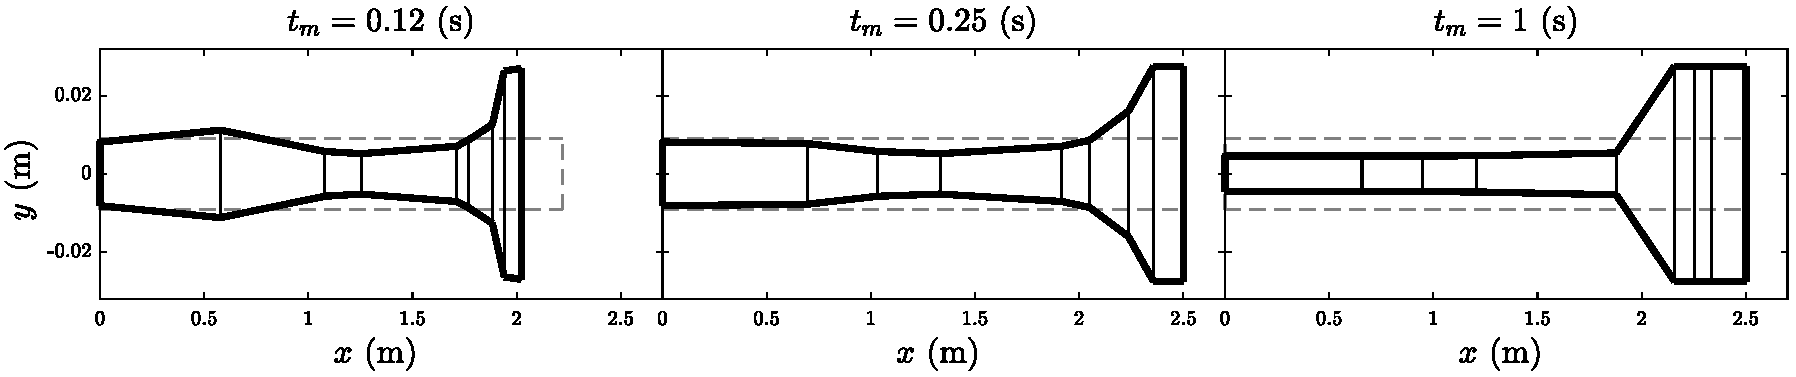
\includegraphics[width=\columnwidth]{../ch7/figures/ArraysPLS.pdf}
      \caption{Array designs for both Variable Length (dashed) and Piecewise Linear Segments (solid) studies.}\label{fig:ch7:arrays_pls}
    \end{subfigure}
    
   \caption{Optimal array designs.}
   
\end{figure}

\begin{figure}[p]
    \centering
    \begin{subfigure}[b]{\textwidth}
      \centering
      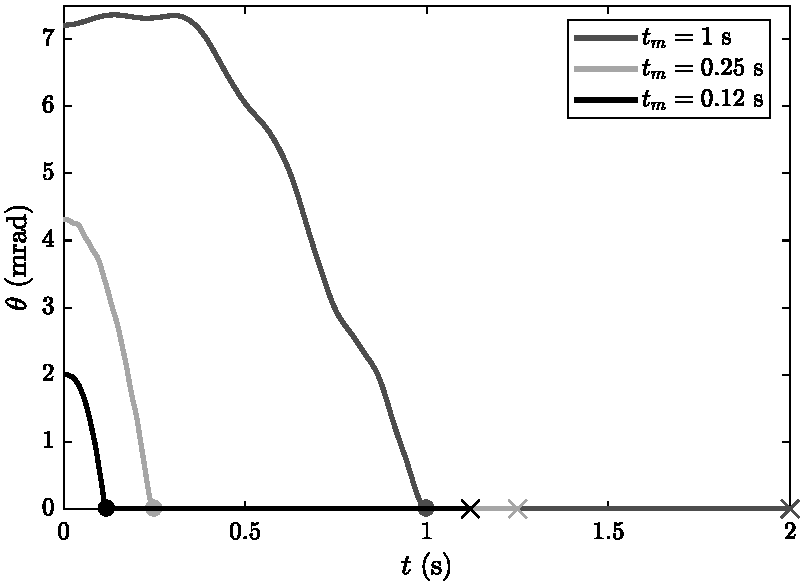
\includegraphics[height=2.2in]{../ch7/figures/ThetasPLS.pdf}%
      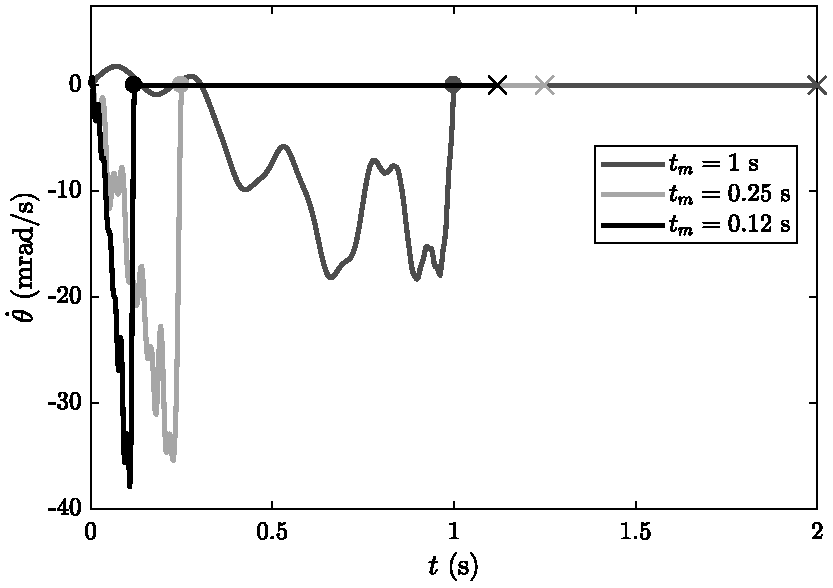
\includegraphics[height=2.2in]{../ch7/figures/dThetasPLS.pdf}%
      \caption{Piecewise Linear Segments (PLS).}\label{fig:ch7:thetas_pls}
    \end{subfigure}
    \begin{subfigure}[b]{\textwidth}
      \centering
      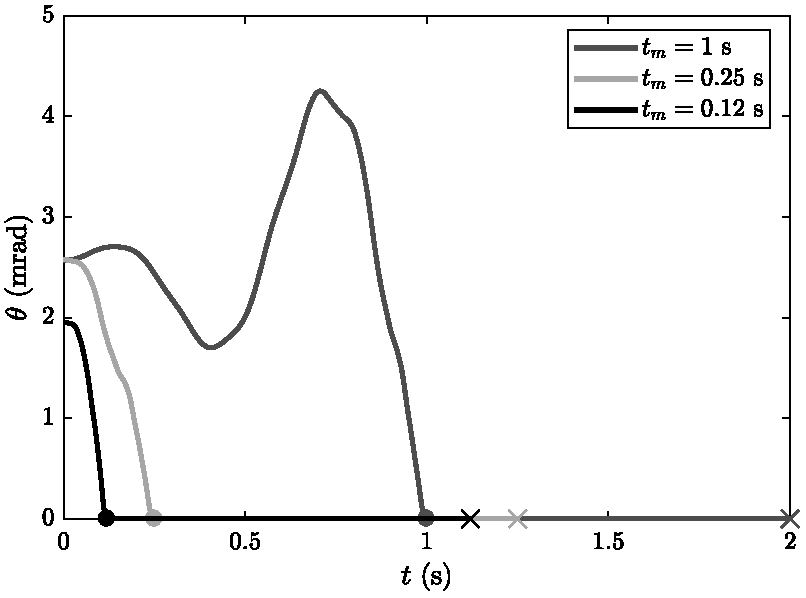
\includegraphics[height=2.2in]{../ch7/figures/ThetasVL.pdf}%
      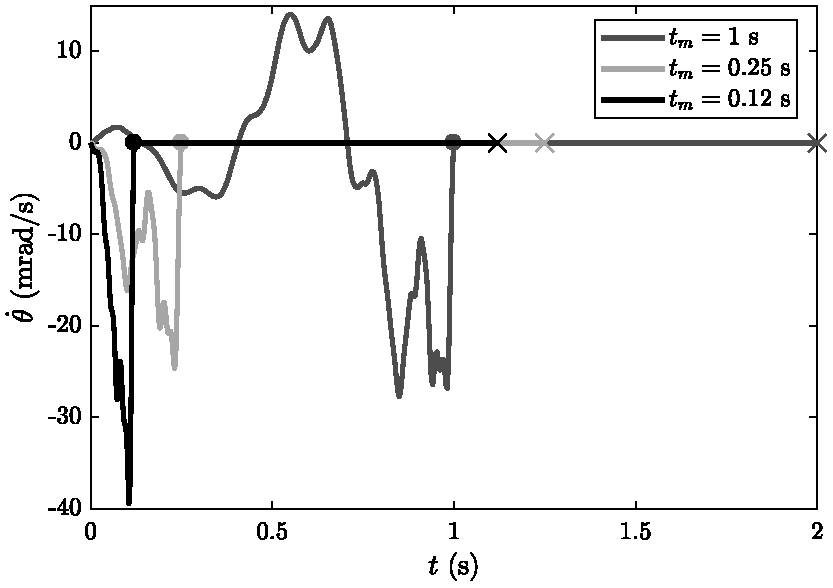
\includegraphics[height=2.2in]{../ch7/figures/dThetasVL.pdf}%
      \caption{Variable Length (VL).}\label{fig:ch7:thetas_vl}
    \end{subfigure}
    \caption{Bus angle and angular rate trajectories for select values of $\bar{t}$.\label{fig:ch7:thetas}}
\end{figure}

\begin{figure}[p]
    \centering
    \begin{subfigure}[b]{0.85\textwidth}
      \centering
      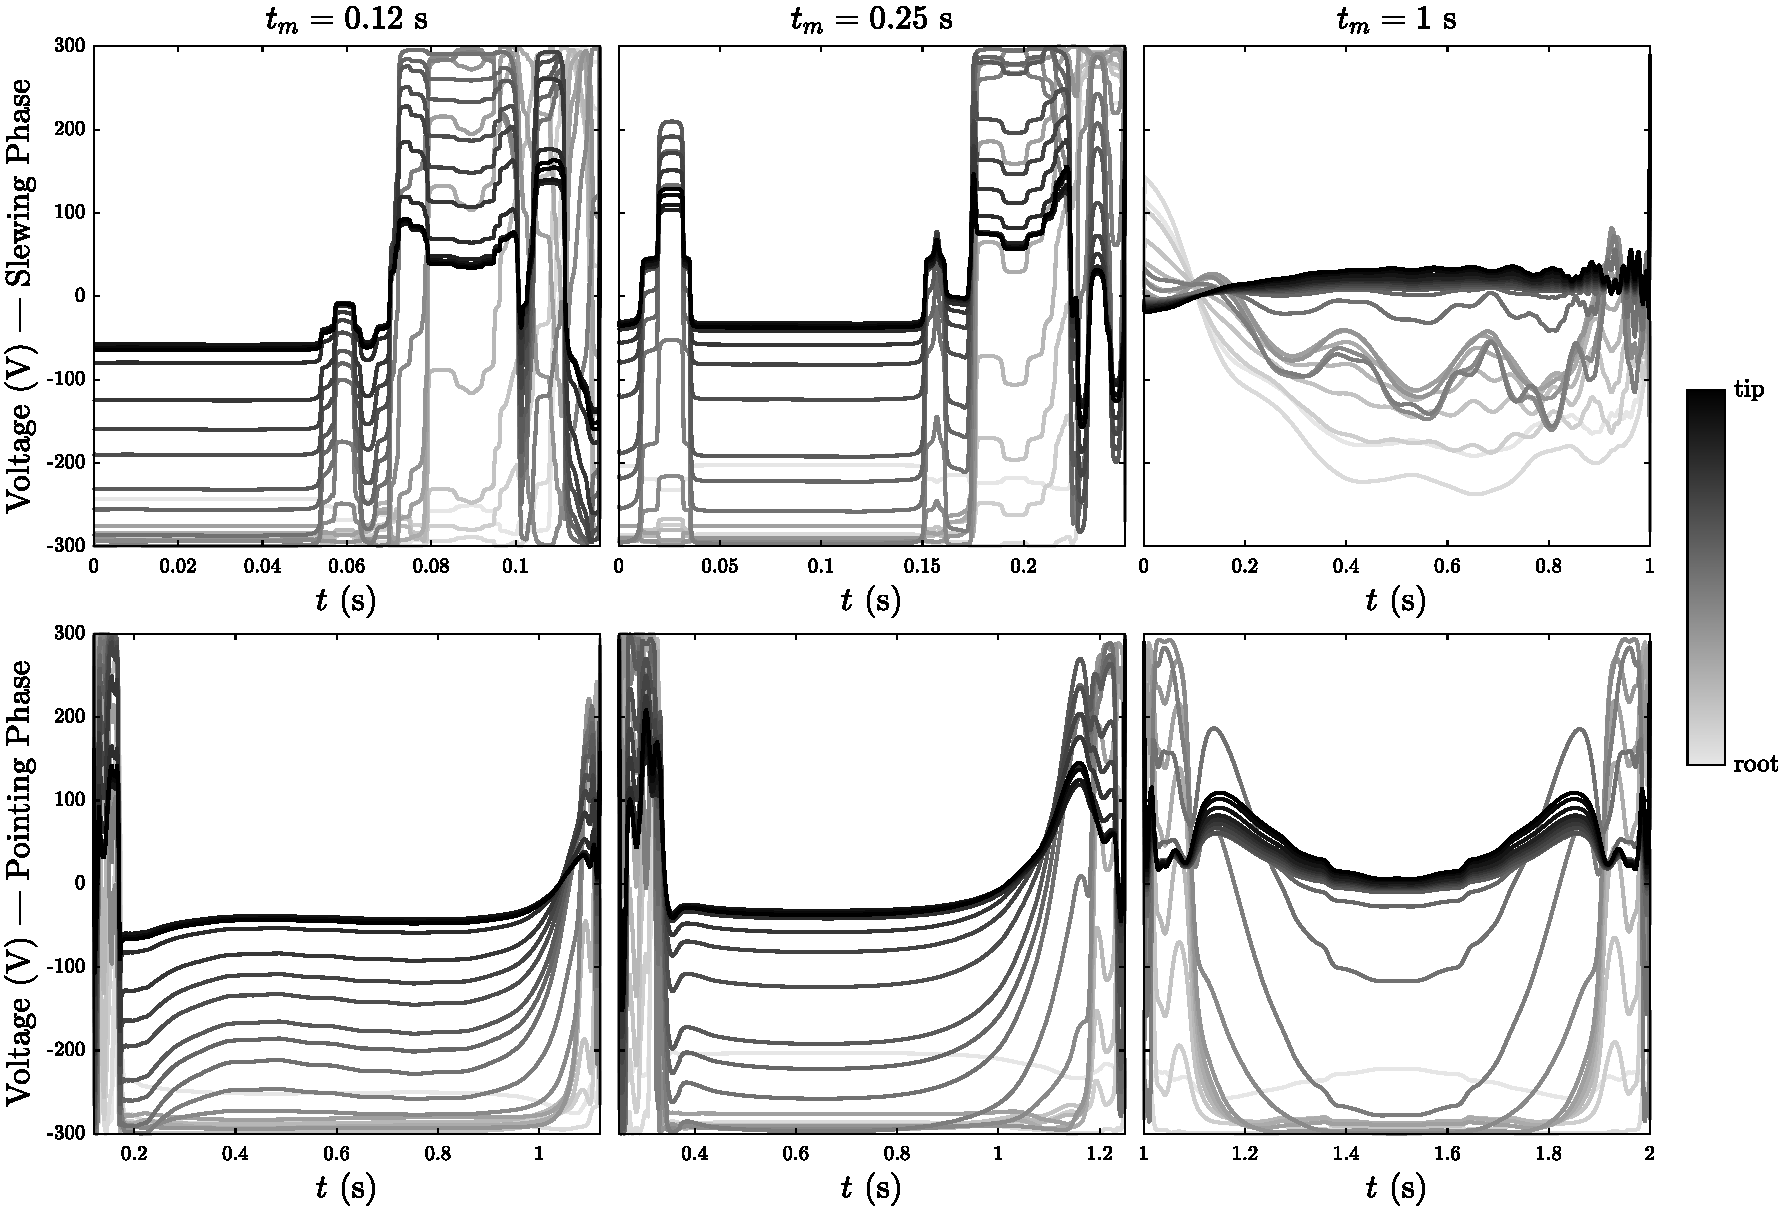
\includegraphics[width=\columnwidth]{../ch7/figures/VoltagePLS.pdf}
      \caption{Piecewise Linear Segments (PLS).} \label{fig:ch7:voltage_pls}
    \end{subfigure}
    \begin{subfigure}[b]{0.85\textwidth}
      \centering
      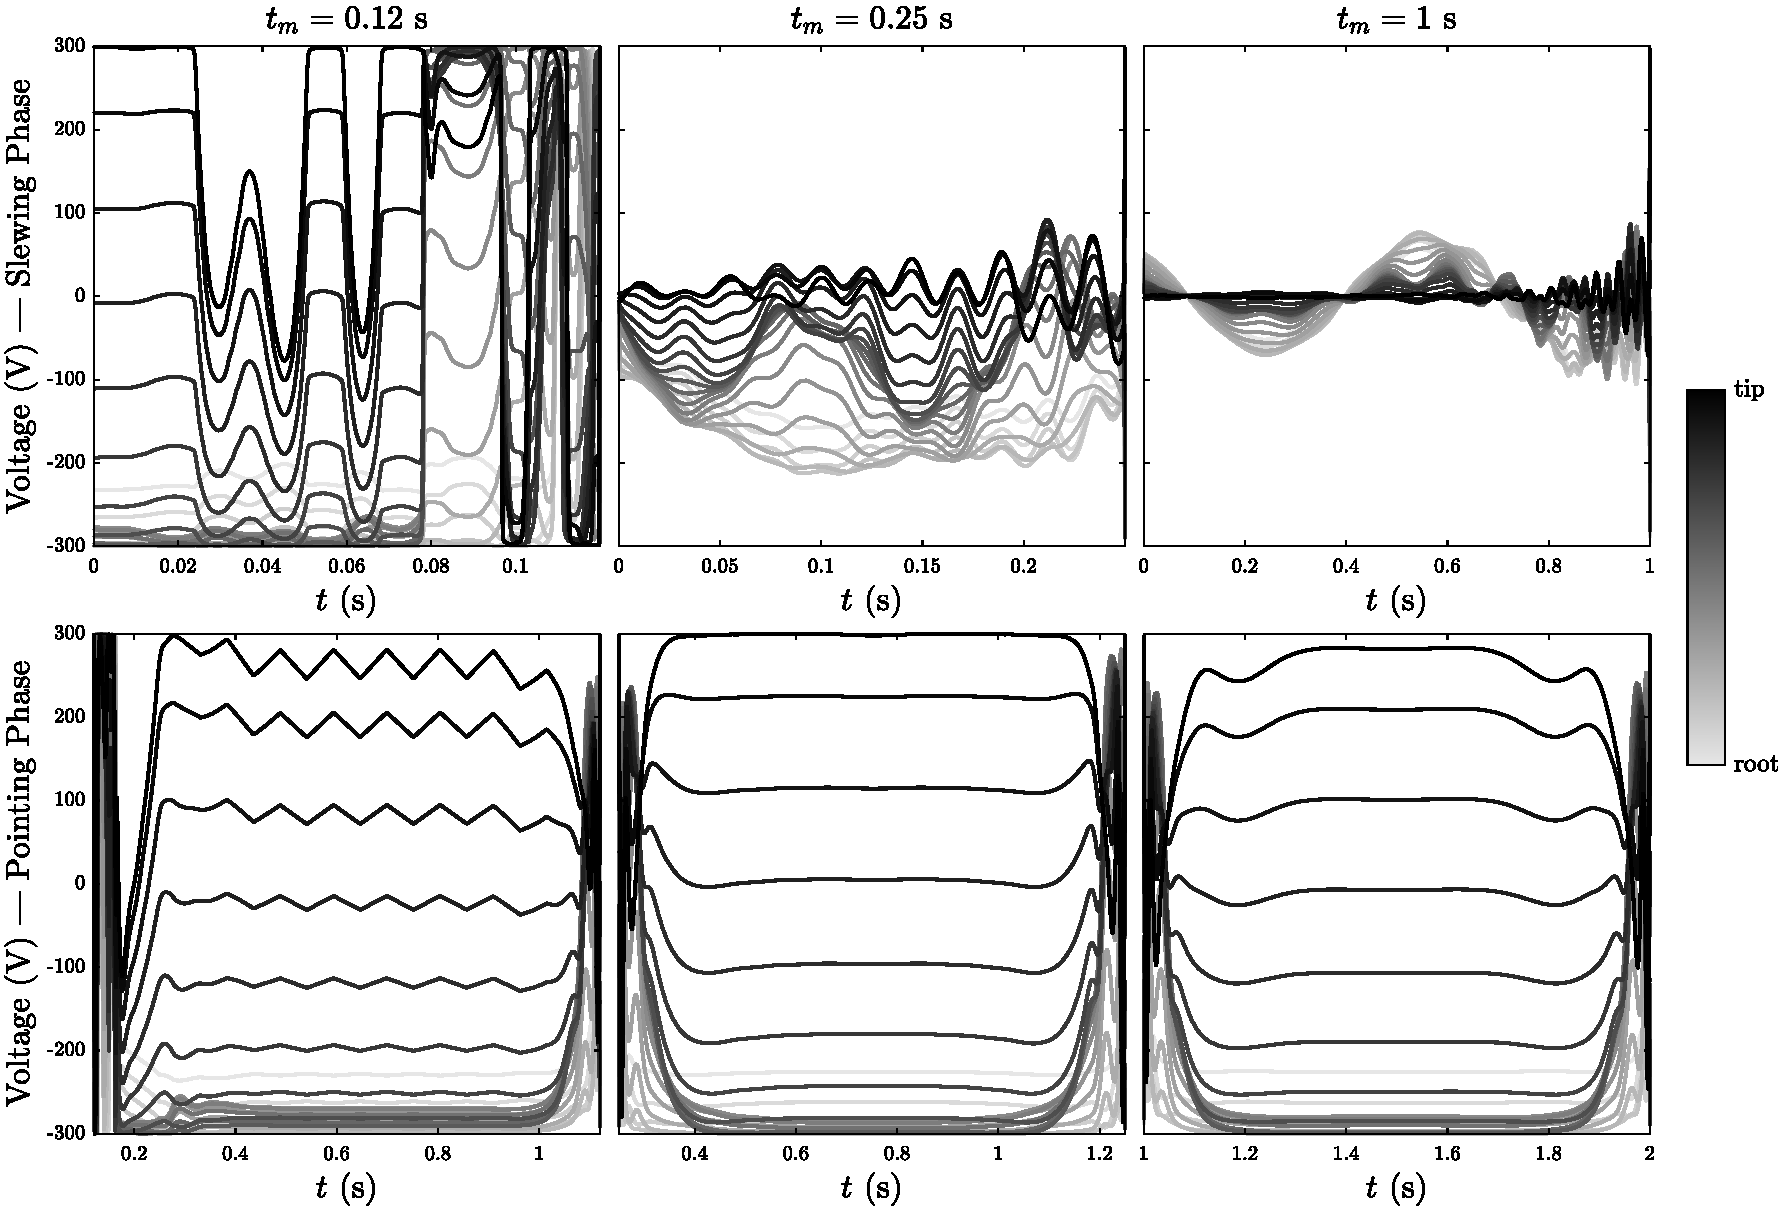
\includegraphics[width=\columnwidth]{../ch7/figures/VoltageVL.pdf}
      \caption{Variable Length (VL).} \label{fig:ch7:voltage_vl}
    \end{subfigure}
    \caption{Voltage history along the array for select values of $\bar{t}$.\label{fig:ch7:voltage}}
\end{figure}

The array displacements for the PLS and VL cases are shown in Fig.~\ref{fig:ch7:displacement}. Results from slewing and pointing phases are shown separately. Conservation of angular momentum with negligible material damping in the bus-array system provides a natural explanation of these numerical results. For example, rotating the bus in the clockwise direction requires the array to displace in the opposite direction (counter-clockwise) (see Fig.~\ref{fig:ch7:coordinate}). This is particularly evident in the VL case with slewing time of 1.0 sec, which shows the effect of CW and CCW array displacements on the bus angle trajectory in Figs.~\ref{fig:ch7:displacement_vl} and~\ref{fig:ch7:thetas_vl}.

\begin{figure}[p]
    \centering
    \begin{subfigure}[b]{0.85\textwidth}
      \centering
      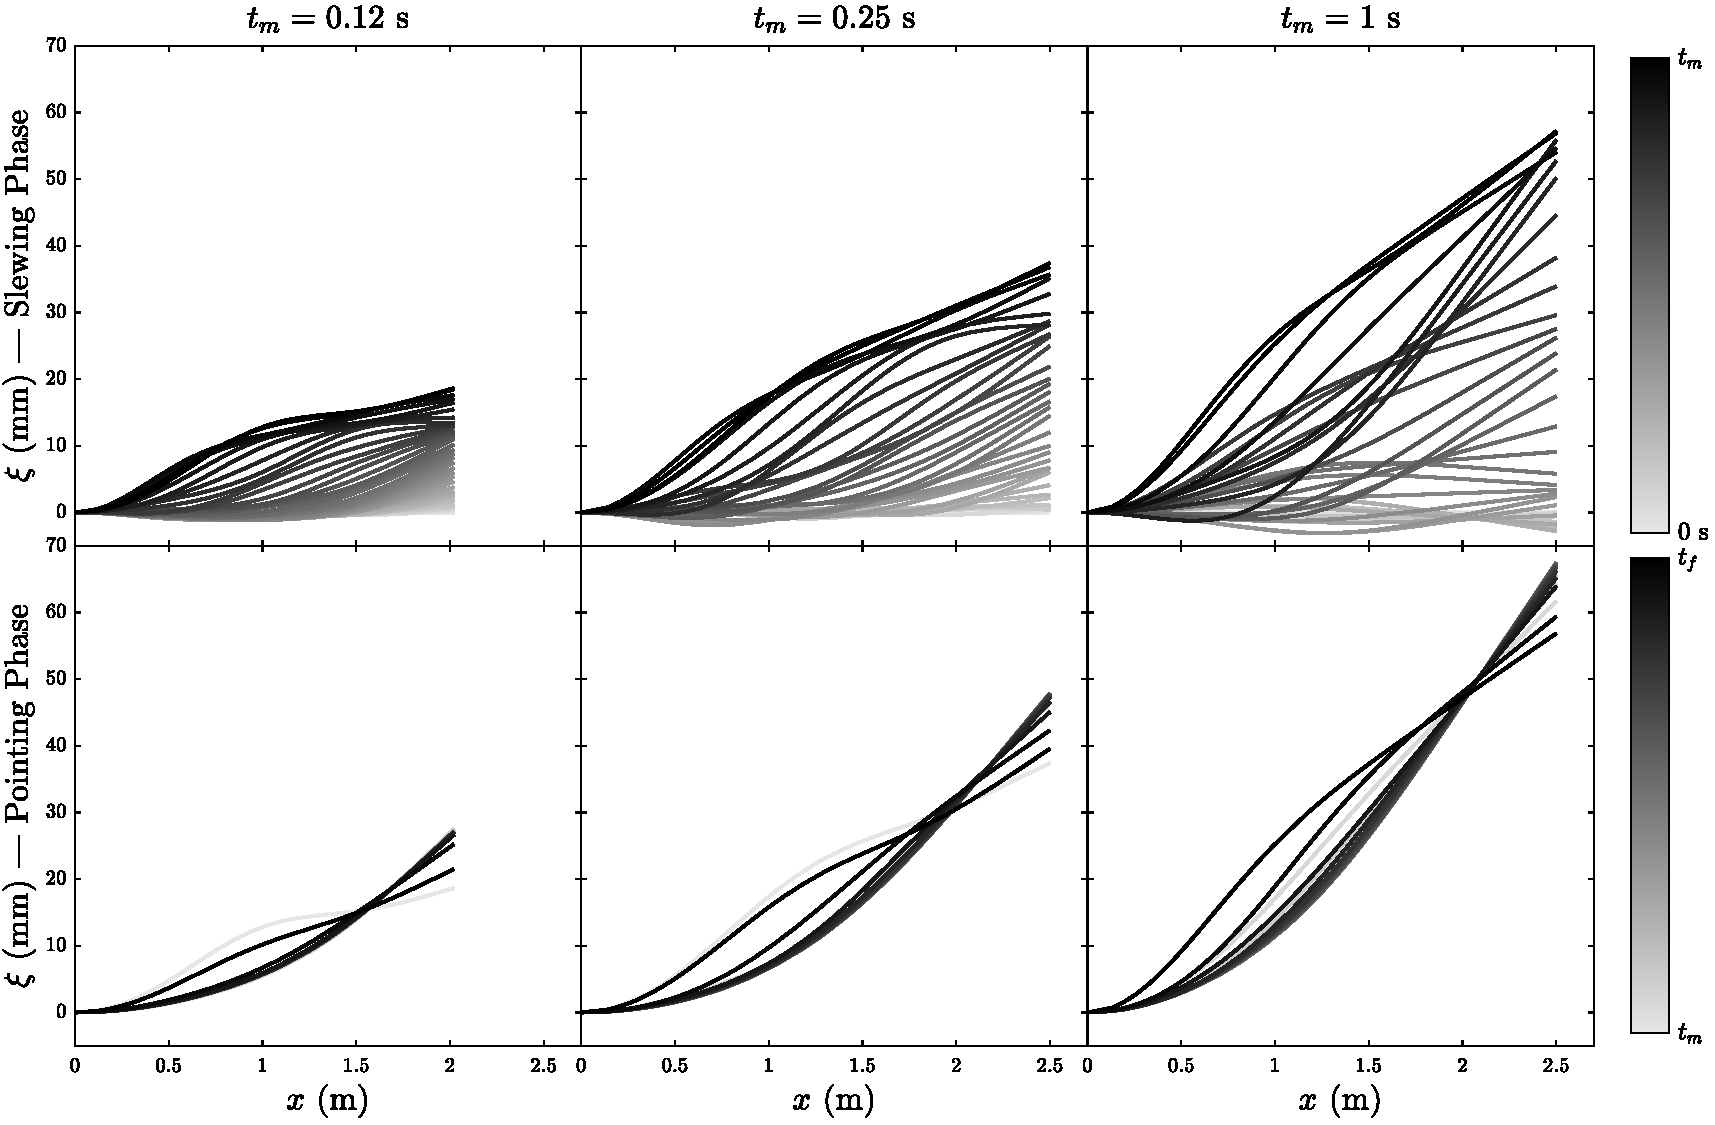
\includegraphics[width=\textwidth]{../ch7/figures/DisplacementPLS.pdf}
      \caption{Piecewise Linear Segments (PLS).}\label{fig:ch7:displacement_pls}
    \end{subfigure}
    \begin{subfigure}[b]{0.85\textwidth}
      \centering
      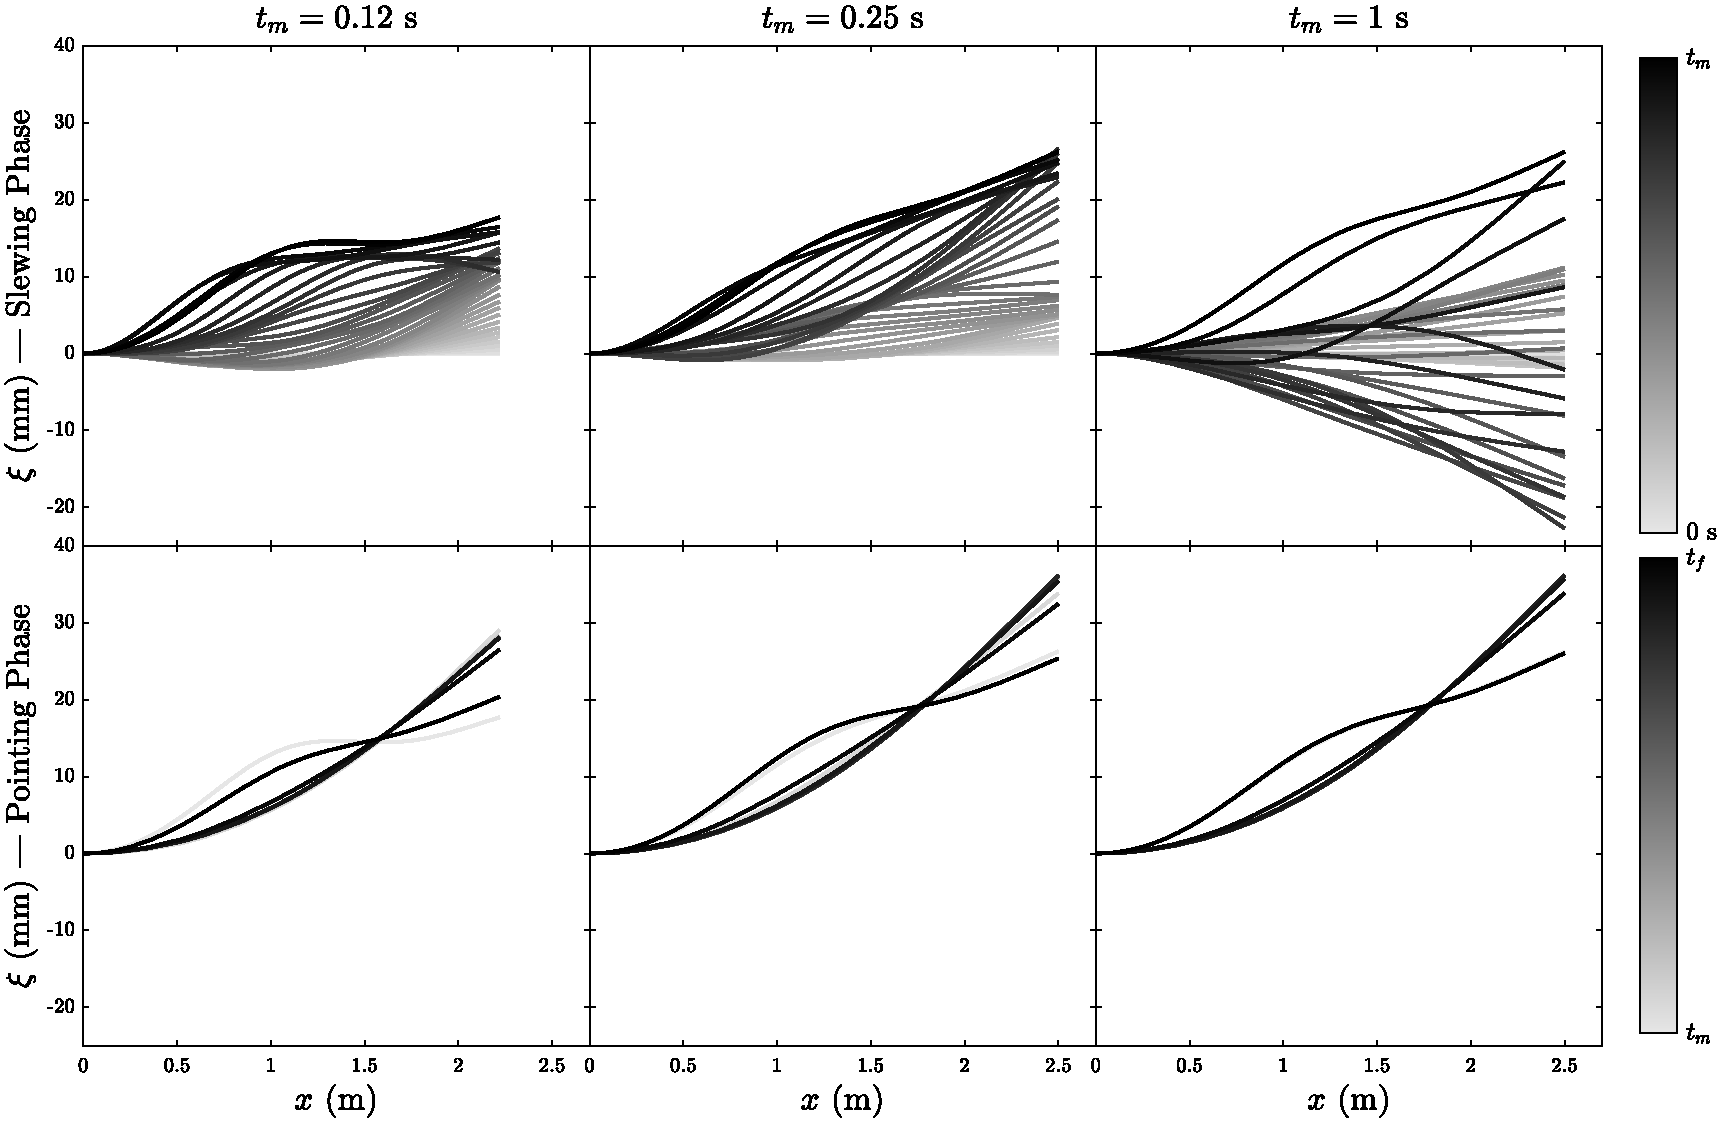
\includegraphics[width=\textwidth]{../ch7/figures/DisplacementVL.pdf}
      \caption{Variable Length (VL).}\label{fig:ch7:displacement_vl}
    \end{subfigure}
    \caption{Array deflection profiles for select values of $\bar{t}$.\label{fig:ch7:displacement}}
\end{figure}

Figure~\ref{fig:ch7:arrays_pls} shows the array physical design evolution with respect to the slewing time. For longer slewing times ($\geq 0.5$~s for the PLS case and $\geq 0.25$~s for the VL case), the optimal array design maximizes the effective inertia ratio between the bus and the arrays subject to the given constraints. This array shape also corresponds to the maximum slew limits seen in the parametric study confirming the general result shown in Sec.~\ref{sec:ch7:prbdm_bounds}. With this observation, we could define a cost proxy function for maximizing array inertia when we have long slewing times~\cite{Allison2013d}. With shorter slewing times, however, we see more complex designs that do not maximize inertia. Since the analysis using the PRBDM model did not take into account the control system, we need an alternate explanation for these optimal arrays designs. To this end, an integrated analysis is performed that considers the synergy between natural passive dynamics (natural modes of the array, no control) and active (controlled) dynamics.

\subsection{Optimal Design Tradeoff for Array Structure}

The periods of the first natural modes for the array designs of the PLS and VL cases are shown in Fig.~\ref{fig:ch7:periods_pls} (the NG case is not considered as it does not involve any modifications of the physical array design). The dashed line is a reference that indicates whether one quarter of the period of the first natural frequency, denoted $\gls{firstperiod}/4$, is longer (above) or shorter (below) than the given slewing time. We use the $T_{1}/4$ line as a reference but the true relationship for this particular co-design formulation appears to be closer to $T_{1}/4.2$, and likely varies slightly based on problem parameters. Consider now the array design that maximizes the array moment of inertia, subject to the given constraints, for a given problem variation with a particular value for $T_1$. If this particular value for $T_{1}/4$ is shorter than the slewing time, the maximum inertia design will be optimal and the optimal controller will utilize primarily the passive dynamics of the first structural mode to achieve an optimal slewing maneuver (and use higher-order modes partially). If $T_{1}/4$ is longer than the given slewing time, the maximal inertia array design can only make partial use of the first mode dynamics in the slewing direction during the given slewing horizon. In other words, the array dynamics now need to be faster to work synergistically with the active controller when the slewing time is reduced, and the relationship between $t_m$ and $T_1$ is approximately linear due to simple scaling of the problem based on the time horizon (see Sec.~\ref{sec:ch4:sasa} for the scaled problem and a discussion on this finding). 
Co-design studies are ideal for determining this tradeoff since allowing simultaneous structural and control design freedom provides access to higher performance levels through synergistic structural and control design tailoring without major assumptions, i.e.,~the parameters for the array structure and open-loop control design are distributed. These results also reveal that the proxy objective function of maximizing inertia is not accurate for faster slew times.

In the cases where the optimal tradeoff is active, the optimal control trajectories include a bang-bang control near the root during the slewing phase, and the optimal array structure changes according to the given design freedom in Table~\ref{tb:ch7:parametric_study}. For the VL case, the only mechanism available for changing inertia and the first natural frequency is to adjust $\ell$, explaining the observed shorter array when $t_m = 0.12$ s (see Fig.~\ref{fig:ch7:arrays_pls}). For the PLS case, the inertia and the first natural frequency are changed by redistributing the mass and/or reducing the array length to utilize more fully a combination of the array's elastic and inertial properties. Observe that the array mass is not reduced, i.e.,~the mass constraint in Eqn.~(\ref{eq:ch7:volume_con}) is active. In addition to using the first natural mode, results indicate that the optimal solutions with shorter $t_m$ also tend to leverage the use of the second natural mode (refer to the increase in the coefficient of the second mode in Fig.~\ref{fig:ch7:modes}). Tailoring of the structural design to best use the second mode is evident by the placement of a segment with local minimum thickness near the midpoint of the array length in Fig.~\ref{fig:ch7:arrays_pls}. The additional structural design freedom provided by the PLS formulation vs.~the VL formulation demonstrates the ability of a co-design formulation with more plant design freedom to tailor the passive dynamics of the system to achieve better performance \cite{Allison2013d}.

\begin{figure}[t]
\centering
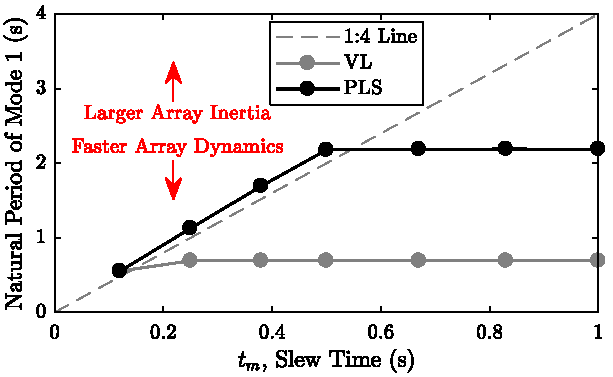
\includegraphics[width=0.6\columnwidth]{../ch7/figures/PeriodSlew}
\caption{Comparison between the first natural period of the optimal array designs and the slewing phase duration.}\label{fig:ch7:periods_pls}
\end{figure}

\begin{figure}[t]
    \centering
    \begin{subfigure}[b]{0.98\textwidth}
      \centering
      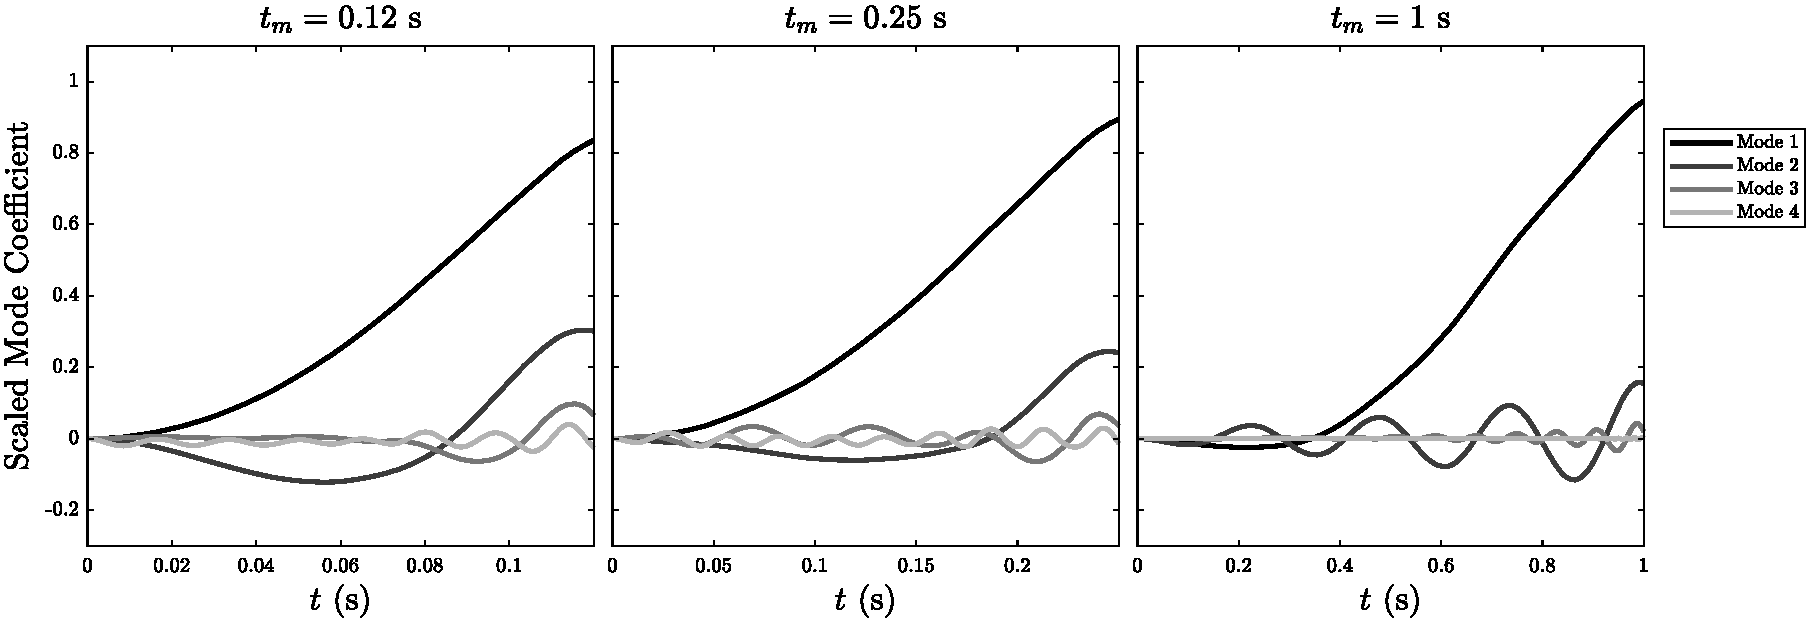
\includegraphics[width=\columnwidth]{../ch7/figures/ModesPLS}
      \caption{Piecewise Linear Segments (PLS) design results.}\label{fig:ch7:modes_pls}
    \end{subfigure}
    \begin{subfigure}[b]{0.98\textwidth}
      \centering
      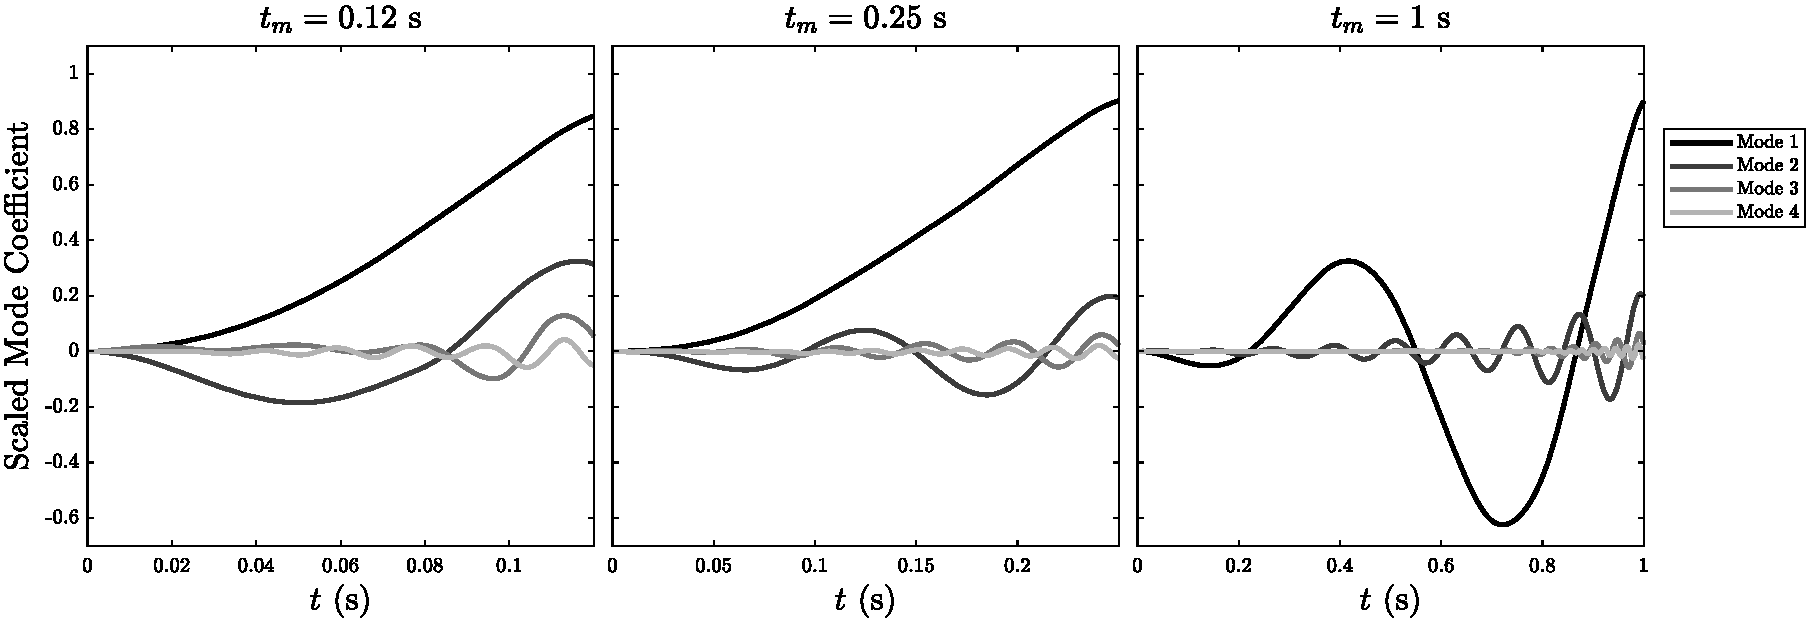
\includegraphics[width=\columnwidth]{../ch7/figures/ModesVL}
      \caption{Variable Length (VL) design results.}\label{fig:ch7:modes_vl}
    \end{subfigure}
    \caption{Scaled mode coefficient trajectories for select values of $\bar{t}$.\label{fig:ch7:modes}}
\end{figure}

\begin{figure}[ht]
    \centering
    \begin{subfigure}[b]{\textwidth}
      \centering
      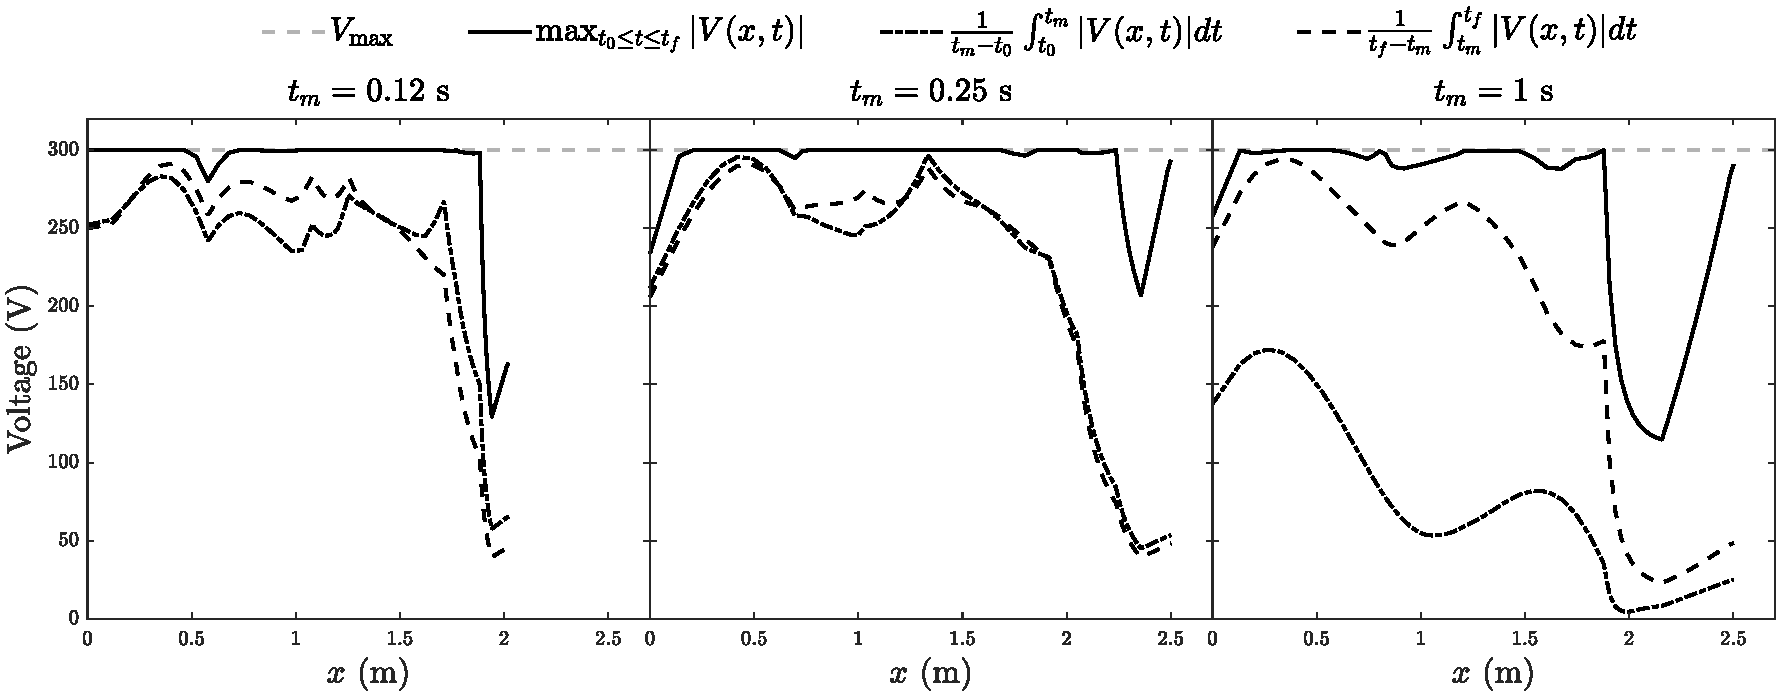
\includegraphics[width=\columnwidth]{../ch7/figures/VoltageStatsPLS.pdf}
      \caption{Piecewise Linear Segments (PLS) design results.}\label{fig:ch7:voltage_stats_pls}
    \end{subfigure}
    \begin{subfigure}[b]{\textwidth}
      \centering
      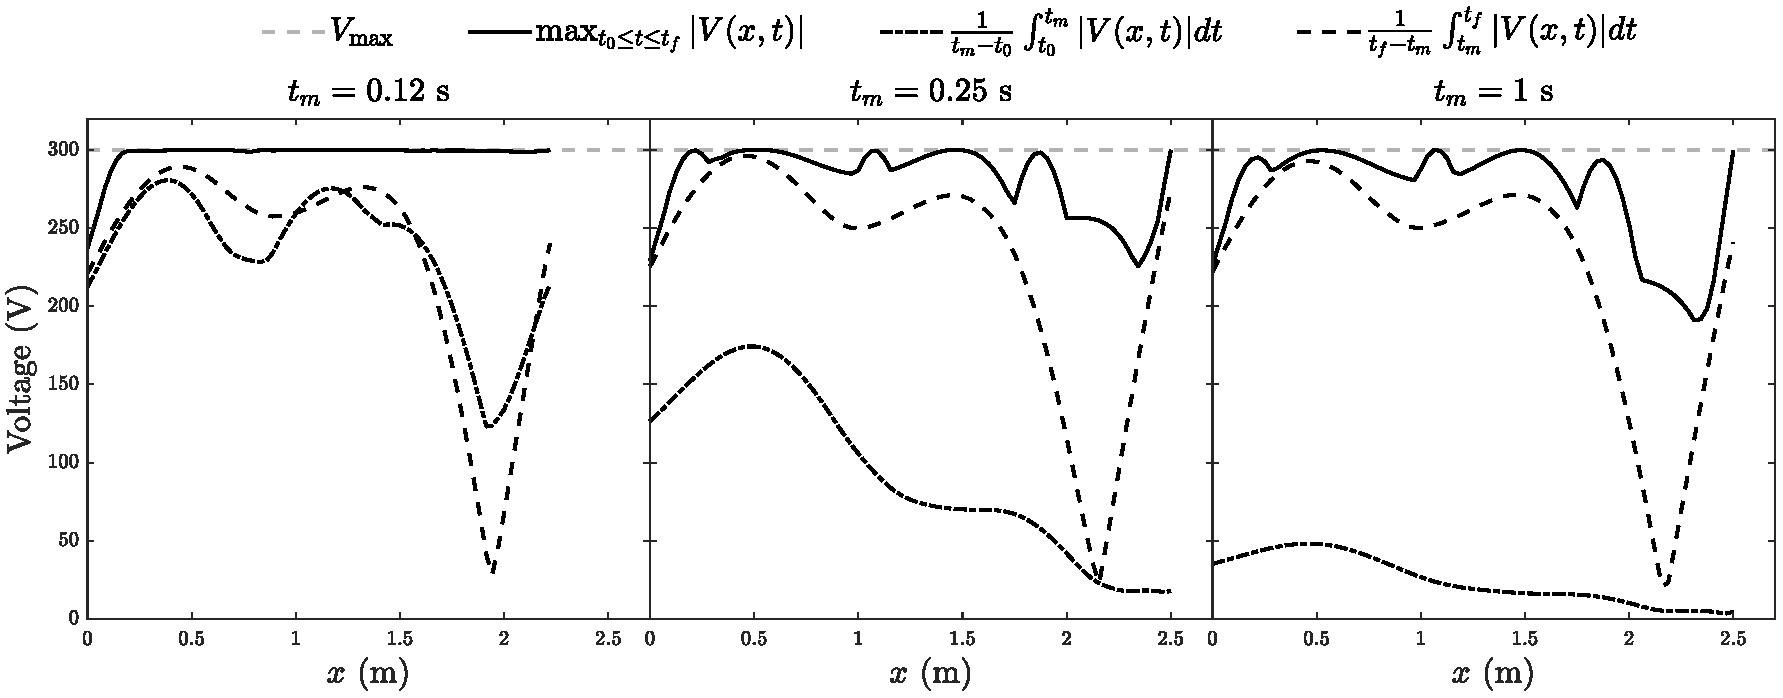
\includegraphics[width=\columnwidth]{../ch7/figures/VoltageStatsVL.pdf}
      \caption{Variable Length (VL) design results.}\label{fig:ch7:voltage_stats_vl}
    \end{subfigure}
    \caption{Voltage trajectory metrics for select values of $\bar{t}$.\label{fig:ch7:voltage_stats}}
\end{figure}

\subsection{Optimal Placement of Segmented Piezoelectric Actuators \label{sec:ch7:placement}}

A continuously variable, spatially distributed voltage is not a physically realizable actuation strategy, but these optimal trajectories provide insights into performance limits, as well as how a physically realizable strain actuation system should be designed. Continuous voltage variation can be approximated using several piezoelectric segments as shown in Fig.~\ref{fig:ch7:varbeam-d-ut}, where a constant voltage $V_i(t)$ is applied to each segment. An analysis of optimal voltage trajectories for the PLS and VL cases was performed to provide insight into actuator placement. Figure~\ref{fig:ch7:voltage_stats} illustrates for each spatial position along the array 1) the maximum voltage amplitude across all time, 2) the mean voltage amplitude during slewing, and 3) the mean voltage amplitude during pointing. The maximum allowable voltage magnitude is 300 $V$. For small $t_m$, the actuators are nearly saturated during the slewing phase, and the voltage limit is reached at some point during the maneuver across most of the array. When the slewing times are longer, the lower average voltage magnitude during the slewing phase is due to the use of modal resonance.

We see that a physical implementation would benefit from placing piezoelectric segments over most of the array area with the exception of the tip. Since each piezoelectric segment can only be actuated with a voltage that is constant in space (not in time), a large number of individual segments translates into more degrees of freedom for the control, which in turn can allow higher performance. However, the voltage metrics suggest that at a minimum two piezoelectric segments should be placed at the two points of local maximum average voltage (which are located near the root and the length midpoint), to take advantage of the natural passive dynamics. These locations are near the critical points of the shapes of the first and second natural modes, which are the dominant modes during the slewing phase as shown in Fig.~\ref{fig:ch7:modes}. The scaled mode coefficients in this figure indicate the relative contribution of each mode in their linearly combined effect on the array deflection. Future studies can include model actuation using individual piezoelectric segments with constant spatial voltage and limited length to determine their optimal placement location. 

\section{Summary\label{sec:ch7:conclusions}}

In this chapter, we investigated the integrated structural and control system design of a strain-actuated solar array for spacecraft pointing control and jitter reduction. Slew maneuvers on the order of milli-radians or arc minutes have been achieved in simulations for a representative spacecraft system without increasing the total array mass or reducing the array planform area. A parametric study was conducted with different levels of design freedom and slewing times. Results show that separately designing the control system or the structural system alone cannot achieve the higher performance levels that are possible through the proposed combined design of the structural and control systems. Furthermore, adding degrees of freedom to the structural design---specifically, distributed geometric design---improved performance further by tailoring the passive dynamics of the array with the active controller.
This study also indicated the relative effectiveness of the nested co-design strategy over the simultaneous one for certain design problems.

Since the SASA system is based on internal actuation, the angular momentum of the bus-array system must be conserved in the absence of material or joint damping. A desired bus rotation requires array deflection in the opposite direction. Results showed that in addition to accomplishing the required slewing and pointing maneuvers, the optimal array design is driven by the interaction between active and natural passive dynamics. Conservation analysis indicates that increasing the array moment of inertia helps improve the maximum slewing angle. An array design with maximum mass moment of inertia subject to the given constraints will be optimal if the slewing horizon is larger than a problem-dependent scaling of the first natural mode period of the array (approximately one quarter of this period), and the optimal controller will use modal resonance for an efficient slewing maneuver. For faster slew maneuvers, however, structural dynamics analysis reveals that it is beneficial to choose a tailored design that reduces inertia somewhat, but provides faster passive dynamics that interact with active control to increase the maximum slew angle. The optimal design here occurs when approximately one quarter of the period of the first natural mode is equal to the slewing time. This allows the passive dynamics to contribute to the maximization of the displacement of the first natural mode in the given slewing horizon, which in turn maximizes the slewing angle. In these cases, the resulting control design includes a bang-bang control near the root during the slewing phase. Results also show that the dynamic behavior of the array may be approximated by a PRBDM system with rigid links and joints. This connection helped provide qualitative insights into the design and behavior of intelligent structures with distributed actuation.